\documentclass{EPL-master-thesis-covers-FR}

\title{HaïtiWater 2.0}
\subtitle{Evolution de l'application HaïtiWater vers une application entière  fonctionnelle hors-ligne}

\author{Vincent \textsc{Gradzielewski}}% Handcrafted third author :D

\degreetitle{Master [120] en sciences informatiques}

\supervisor{Kim \textsc{Mens}}
\secondsupervisor{Sandra \textsc{Soares-Frazão}}

\readerone{}
\readertwo{}

\years{2020-2021}

\usepackage{subcaption}
\captionsetup{compatibility=false}
\usepackage{hyperref}
\usepackage{cite}
\usepackage{float}
\usepackage{multirow}
\usepackage{multicol}
\usepackage[final]{pdfpages}
\usepackage{booktabs}
\usepackage{multirow}
\usepackage{graphicx}
\usepackage[toc]{multitoc}
%Vérifier la table des matière (une colonne)

\usepackage{amssymb}% http://ctan.org/pkg/amssymb
\usepackage{pifont}% http://ctan.org/pkg/pifont
\newcommand{\cmark}{\ding{51}}% pour les checkmark
\newcommand{\xmark}{\ding{55}}%

\frenchbsetup{StandardLists=true} % Resolves conflict between babel and enumitem
\usepackage{enumitem} % better formating of lists

\usepackage[style=long,nonumberlist,toc,xindy,acronym,nomain]{glossaries}
%Vé
\makenoidxglossaries
	\newacronym{pwa}{PWA}{Progressive Web App}
	\newacronym{sem}{SGBD}{Systeme de Gestion de Base de Données}
	\newglossaryentry{full_stack}{name={full-stack},  description={Développement à la fois sur le fontend et le backend}} 

\begin{document}

	\maketitle
	\tableofcontents

	\setlength{\parskip}{1.5em plus1em minus1em}

	% Total des pages : entre 49 et 75 d'après nos estimations.

	\chapter*{Résumé}
	\addcontentsline{toc}{chapter}{Résumé}
	
		%Objectif, solution, évaluation
	
		Ce travail de fin d'études a été réalisé dans le cadre de mon Master en Sciences Informatiques à l'École Polytechnique de Louvain durant l'année académique 2020-2021 en partenariat avec l'ONG Protos.
		
		Dans ce mémoire, je vais vous présenter mon travail qui consistait à reprendre l'application HaïtiWater développée précedemment par Adrien Hallet, Céline Deknop et Sébastien Strebelle qui a pour nom "La gestion du réseau de distribution d'eau potable en Haïti" \cite{ref:haitiwater}. Le but de ce travail est de transformer cette web-application pour qu'elle soit entièrement utilisable \textbf{lorsque la connexon au serveur n'est pas disponible}.
	
		Cette application a pour but "La gestion du réseau de distribution d'eau potable en Haïti". Je commencerai par une brève introduction sur le contexte Haitien et sur les raisons pour lesquelles l'évolution de cette application était nécessaire. Ensuite je présenterai le principe des \gls{pwa} et pourquoi j'ai choisis d'utiliser cette technologie plûtot qu'une autre. Je présenterai par après la validation de l'application et les feedback que j'ai reçu des utilisateurs. Puis je concluerai par une liste des améliorations possibles pour le futur développement de l'application.

		Tout le code source de l'application est disponible à cette adresse : \url{https://github.com/exavince/HaitiWater}

		Si vous désirez tester l'application, il suffit de demander un login à une des personnes ayant travaillé sur l'application et de vous rendre sur le lien suivant \url{https://haitiwater.sipr.ucl.ac.be} afin de vous connecter à l'application.
		

	\chapter*{Remerciements}
	\addcontentsline{toc}{chapter}{Remerciements}
		Dans le cadre de ce mémoire, j'ai été aidé par différentes personnes sans lesquelles la réalisation de celui-ci n'aurait pas été possible. Je souhaite donc prendre ces quelques lignes pour les remercier.
		
		Merci aux professeurs Kim Mens et Sandra Soares-Frazão pour leur aide, leur soutient et les conseils indispensables qu'ils m'ont apportés tout au long de ce travail.
		
		Merci à l'ONG Protos qui a amené ce projet.
		
		Merci à Celine Deknop et Sebastien Sterbelle pour l'aide et les conseils qu'ils m'ont apportés à différent moment de ce projet.
		
		Merci à Nahomie pour l'aide apportée au début du projet afin de bien mettre en évidence les besoins de l'application.
		
		Merci à tous les utilisateurs qui ont pris du temps pour tester l'application et me donner leur feedback sur celle-ci.
		
		Merci à mes parents et à mes amis qui m'ont soutenu et m'ont motivé tout au long de ce mémoire.

		

	\printnoidxglossary[title=Glossaire, toctitle=Glossaire]
	\glsaddall

	\chapter{Introduction}

		
		\subsection*{Contexte}
		
			Ce mémoire appartient à un projet de développement financé par ARES-CCD avec quelques partenaires tels que Protos, l'UCL et l'UEH. L'objectif du ce projet est de réaliser un système logiciel pilote pour la gestion de la distribution d'eau potable en zone rurale. C'est pour cette raison que l'ONG Protos est active en Haïti depuis plusieurs années.
			
			Protos est une ONG qui a pour but d'améliorer l'accès à l'eau potable dans plusieurs pays du monde afin de les aider à se développer. Suite à de nombreuses crises politiques et catastrophes naturelles qui ont détruit beaucoup d'infrastructures locales, l'accès à l'eau potable est devenu difficile en Haïti. De plus, des incertitudes politiques entravent la reconstruction de ces installations et les populations ne sont pas toujours aidées par les services publiques pour assurer la distribution de l'eau. 
			
			 En effet, aucune gestion centralisée et organisée par l'état n'existe pour les zones rurales éloignées des grandes agglomérations. Des réseaux existent, constitués de points de prélèvement d'eau, de conduites de distribution d'eau et de fontaines situées dans les villages, mais la gestion publique de ceux-ci n'est pas opérationnelle. 

			L'application \cite{ref:haitiwater} créée précédemment propose un appui à ces organismes locaux afin de mieux organiser cette distribution. 

			

		\subsection*{Problématiques}
			Actuellement, HaïtiWater est une web-application prévue pour fonctionner uniquement lorsque le réseau est stable et fonctionnel. Malheureusement en Haïti la connexion au réseau internet est assez instable et par endroit ce réseau n'est pas disponible du tout. Il faut donc trouver une solution pour que cette application puisse être utilisable et fiable dans les conditions du contexte Haïtien. 


		\subsection*{Motivation}
			J'ai réalisé ce travail dans le cadre de mon Master en Sciences Informatiques. L'objectif de celui-ci est de mettre en application les différentes compétences acquisent durant mes années d'étude sur un projet de grande envergure.
			
			Au delà de mettre mes compétences en pratique, ce travail va me permettre d'acquérir de l'expérience dans le développement d'applications et surtout dans l'utilisation des nouvelles technologies du web. Il va me permettre d'apprendre à me lancer dans un gros projet pré-existant, de me familiariser avec un environment logiciel déja existant et d'y apporter ma touche personnelle.	
			
			Le plus motivant dans l'évolution de cette application étant de savoir qu'il s'agit d'un projet réel avec de vrais acteurs qui vont utiliser cette application sur le terrain une fois que celle-ci sera terminée.

		\subsection*{Objectifs}
			L'objectif de ce mémoire est de proposer une nouvelle version de l'application HaïtiWater afin que celle-ci soie plus adaptée à un usage sur le terrain. Normalement cette nouvelle version devrait être déployée en Haïti cette année et ce sont les acteurs locaux qui devraient reprendre la maintenance et l'évolution de celle-ci.
			
			Un autre objectif est de délivrer une application propre et stable qui donnera envie aux utilisateurs de l'employer sur le terrain à la place de leurs outils actuels.

			
		\subsection*{Approche}
			Avant de lancer le développement de cette deuxième version de l'application, un gros travail d'analyse a été réalisé afin de déterminer les différentes fonctionnalités à implémenter et la technologie à utiliser. L'analyse de Moscow \cite{ref:moscow} a été utilisée à cette fin.
		
			Après cette phase d'analyse, je me suis lancé dans la phase de développement durant laquelle j'ai implémenté toutes les fonctions décrites lors de la phase d'analyse. C'est cette phase qui a pris le plus clair du temps étant donné le nombre de fonctions à implémenter et la nécessité de faire de la documentation pour les futurs développeurs.
			
			Pour finir vient la phase de validation. L'application a été présentée à des utilisateurs ayant déjà essayé la première version de l'application ou non afin que ceux-ci puissent fournir le feedback nécessaire à l	 future évolution de l'application.
			
		\subsection*{Contribution}
			Grâce au travail réalisé, Protos et les acteurs locaux Haïtiens vont pouvoir déployer l'application et l'utiliser sur le terrain même dans les zones les plus rurales. En effet celle-ci peut maintenant être utilisée lorsque le réseau n'est plus disponible. Pour l'instant ces acteurs utilisent des outils basiques tel que le crayon/papier pour faire leurs rapports sur le terrain, cela ne permet pas d'avoir un accès facile aux informations passées et cela complique beaucoup la transmission de l'information à la hiérarchie. L'utilisation de l'application permettrait de résoudre ces deux problèmes.
			
			J'espère avoir apporté ma contribution à une meilleure gestion de l'eau en Haïti en aidant à la création de cette application. De mon côté, ce travail m'aura permis d'acquérir de nouvelles compétences dans développement full stack d'appliactions web.

		\subsection*{Plan}
			Dans ce mémoire, je vais décrire le façon dont s'est déroulé ce travail. Pour commencer je vais faire un bref résumé du contexte Haïtien ainsi que la description de l'application existante. Par la suite je vais expliquer l'analyse des besoins et les décisions prises pour l'implémentation. Je détaillerai par après la façon dont s'est déroulée la phase de validation et je cloturerai par une présentation des évolutions possibles.
		

	\chapter{Contexte}


		\section{La gestion de l'eau en Haïti}
			\label{sec:situation}
			
				Haïti est l'un des pays les plus pauvres au monde. Il est situé dans une zone géographique où les risques de catastrophes naturelles sont très élevés. Ces intempéries détruisent les infrastructures et empêchent le bon développement du réseaux de distribution d'eau potable. Il y a quelques années, en 2010, le pays a subi un énorme séisme qui a ravagé une bonne partie du territoire. Parmi tous les défis à relever vient celui de la gestion et de la distribution de l'eau potable sur ce territoire, surtout dans les zones les plus rurales. Le climat de la région rendant excessivement difficile l'exploitation directe des cours d'eau, il faut beaucoup d'infrastructures afin de pouvoir assumer la distribution de l'eau potable à tous.
				
				En raison de la grande pauvreté qui règnent sur la plupart de l'île et de gros problèmes organisationnels, il est très difficile de maintenir et de développer le réseau de distribution d'eau potable. Il y a un gros manque de collaboration entre les entités haïtiennes ou entre les villages dû en partie à la communication qui n'est pas du tout optimisée voir inexistante dans certains cas. Dans les zones les plus rurales de l'île, le taux de recouvrement des factures est excessivement faible, jusqu'à 11\%.
				
				Pour toutes ces raisons, l'ONG Protos vient donc en aide à Haïti afin d'aider le service national des eaux à gérer la gestion des infrastructures et la facturation des clients surtout dans les zones les plus rurales.
				
				Si vous désirez plus d'informations sur les problèmes environnementaux, politiques, sociaux ou organisationnels du contexte haïtiens, je vous invite à aller consulter le mémoire d'Adrien Hallet, Céline Deknop et Sébastien Strebelle \cite{ref:haitiwater}.

				%Brève explication sur le contexte Haïtien


		\section{Introduction à l'application}
				Dans le cadre de la situation décrite dans la section \ref{sec:situation}, Protos a fait appel à l'UCL afin de créer une application d'aide à la gestion et la distribution de l'eau potable en Haïti. Une première version de l'application a été développée en 2018-2019 par 3 personnes dans le cadre de leur mémoire \cite{ref:haitiwater}, elle comprend différents modules permettant de faciliter la gestion des infrastructures et les clients qui vont y chercher de l'eau. L'application est basée sur un principe hiérarchique\cite{ref:haitiwater}.
				
				\begin{figure}[H]
					\centering
					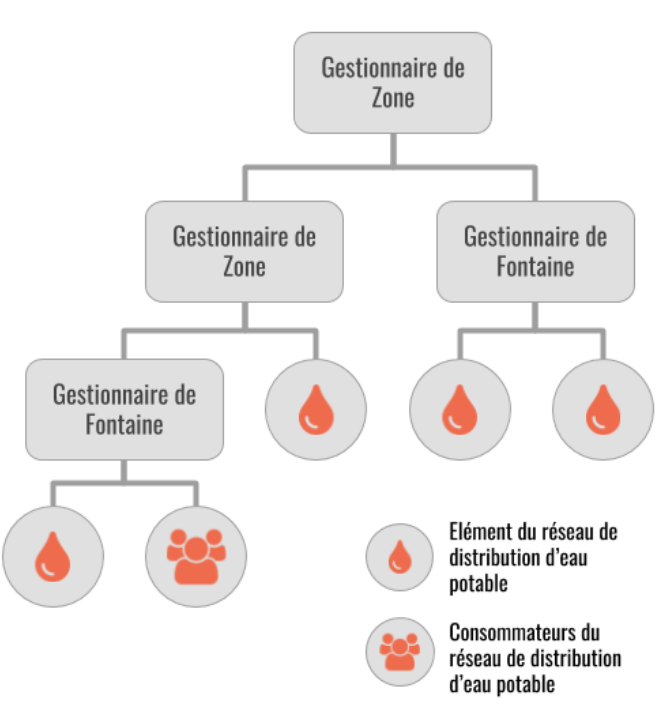
\includegraphics[width=0.5\textwidth]{images/hierarchie}
					\caption{Hiérarchie dans l'application}
				\end{figure}
				
				
			\subsection{Eléments de l'application}
				\begin{description}
					\item[Zone.] Une zone représente une partie du territoire. Elle peut être subdivisée en plusieurs sous-zones, la zone-parent reprendra alors toutes les données des zones enfants. Cela permet de séparer les responsabilités des différents territoires.
					\item[Elements du réseau.] Ces éléments représentent les points physiques du réseau de distribution d'eau potable. Ils sont au nombre de six : conduites, réservoirs, sources, fontaines, kiosques et prises individuelles. Tous ensembles ils forment le réseau de distribution au complet. 
					\item[Consommateurs.] Le consommateur est une personne qui va utiliser le réseau de distribution d'eau potable. Chaque consommateur se voit lors de son enregistrement attribué à un seul élément de sortie d'eau du réseau : fontaine, kiosque, prise individuelle. De cette façon, il est plus simple de gérer la facturation des consommateurs.
				\end{description}
				
			
				
				%Inclusion du schéma zones, fontaines, ... pour rendre la suite plus claire.
				
			\subsection{Utilisateurs de l'application}
				Il y 2 types d'utilisateurs qui peuvent se connecter à l'application
				
				\begin{description}
					\item[Gestionnaire de fontaine.] Ce gestionnaire va gérer la distribution de l'eau aux différents consommateurs. Il devra gérer tous les éléments du réseau qui lui sont attribués.
					\item[Gestionnaire de zone.] Ce gestionnaire va avoir la responsabilité de gérer d'autres gestionnaires de zones et/ou des gestionnaires de fontaines. Son travail est plus d'administrer et de surveiller les personnes qui sont en-dessous de lui.			 
				\end{description}
				
				Ces deux gestionnaires vont avoir des privilèges différents et peuvent donc interagir différemment avec les données. Pour illustrer plus simplement cela, voici un tableau \cite{ref:haitiwater} où vous pourrez retrouver plus d'informations sur les rôles des différents gestionnaires. 
				\begin{table}[H]
					\centering
					\small
					\setlength\tabcolsep{2pt}
					\begin{tabular}{|l|c|c|}
						\hline
						\multirow{2}{*}{\textbf{Permission}} & \multicolumn{2}{l|}{\textbf{Gestionnaire de}} \\ \cline{2-3}
						 & \textbf{fontaine} & \textbf{zone} \\ \hline
						 Ajouter/modifier/supprimer un consommateur & \cmark & \cmark \\ \hline
						 Ajouter/modifier/supprimer un élément du réseau de distribution & \cmark & \cmark \\ \hline
						 Ajouter/modifier/supprimer un rapport mensuel & \cmark & \cmark \\ \hline
						 Ajouter/modifier/supprimer un paiement & \cmark & \cmark \\ \hline
						 Ajouter/modifier/supprimer un ticket de support & \cmark & \cmark \\ \hline
						 Ajouter/modifier/supprimer une zone & \xmark & \cmark \\ \hline
						 Ajouter/modifier/supprimer un gestionnaire & \xmark & \cmark$^{*}$ \\ \hline
						 Accepter/refuser un changement dans l'historique & \xmark & \cmark \\ \hline
						 \multicolumn{3}{p{\textwidth}}{\emph{* : Un gestionnaire de zone ne peut pas modifier les informations personnelles (mot de passe, courrier, nom, prénom) d'un gestionnaire existant}} \\
					\end{tabular}
					\caption{Permissions dans l'application, par type d'utilisateur}
					\label{tab:permissions}
				\end{table}
				
			\subsection{Accueil}
				Ce module contient les informations condensées de la zone qui est attribuée à l'utilisateur. Il peut y retrouver le nombre de fontaines, de kiosques, de points de prises individuelles et de conduites que contient sa zone mais aussi le nombre de foyers et de consommateurs individuels liés à celle-ci. 
								
				\begin{figure}[H]
					\centering
					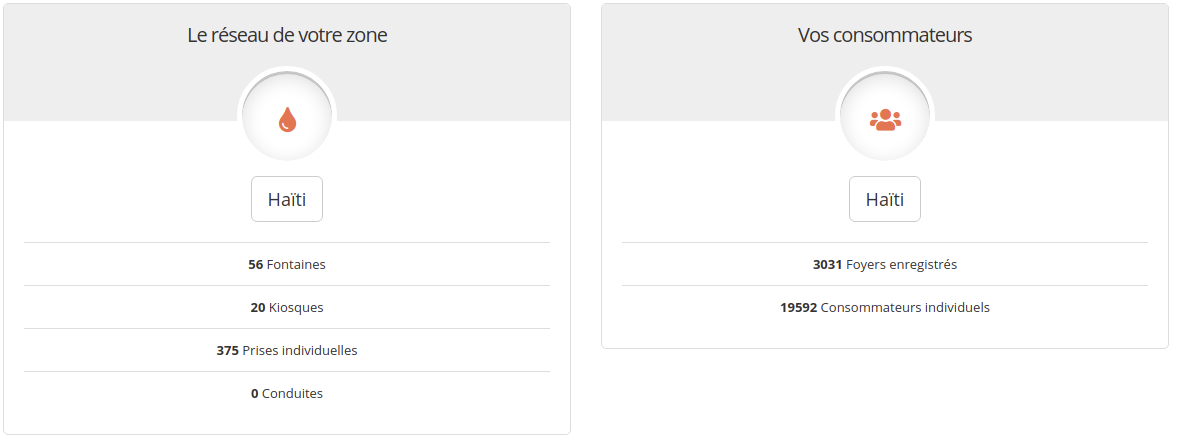
\includegraphics[width=1\textwidth]{images/dashboard}
					\caption{Module d'accueil}
				\end{figure}
				
				
			\subsection{Réseau}
				\label{sec:reseau}
				Dans ce module, l'utilisateur peut retrouver 3 éléments différents.
				
				\begin{description}
				\item[Schéma] Un schéma contenant la répartition des consommateurs par genre ou le volume d'eau mensuel distribué dans chaque zone. Il peut sélectionner le schéma à afficher grâce à une liste déroulante.
				\item[Résumé de zone] Un résumé de sa zone géographique contenant le nombre de consommateurs et de points d'eau présents ainsi que le volume d'eau distribué dans celle-ci.
				\item[Elements du réseau] Un tableau interactif qui contient tous les différents éléments du réseau. Dans cette partie en fonction de ses privilèges, celui-ci peut supprimer, modifier ou ajouter des éléments du réseau. Il peut également trier ou faire des recherches dans ce tableau selon ses besoins.
				\end{description}
				
				\begin{figure}[H]
					\centering
					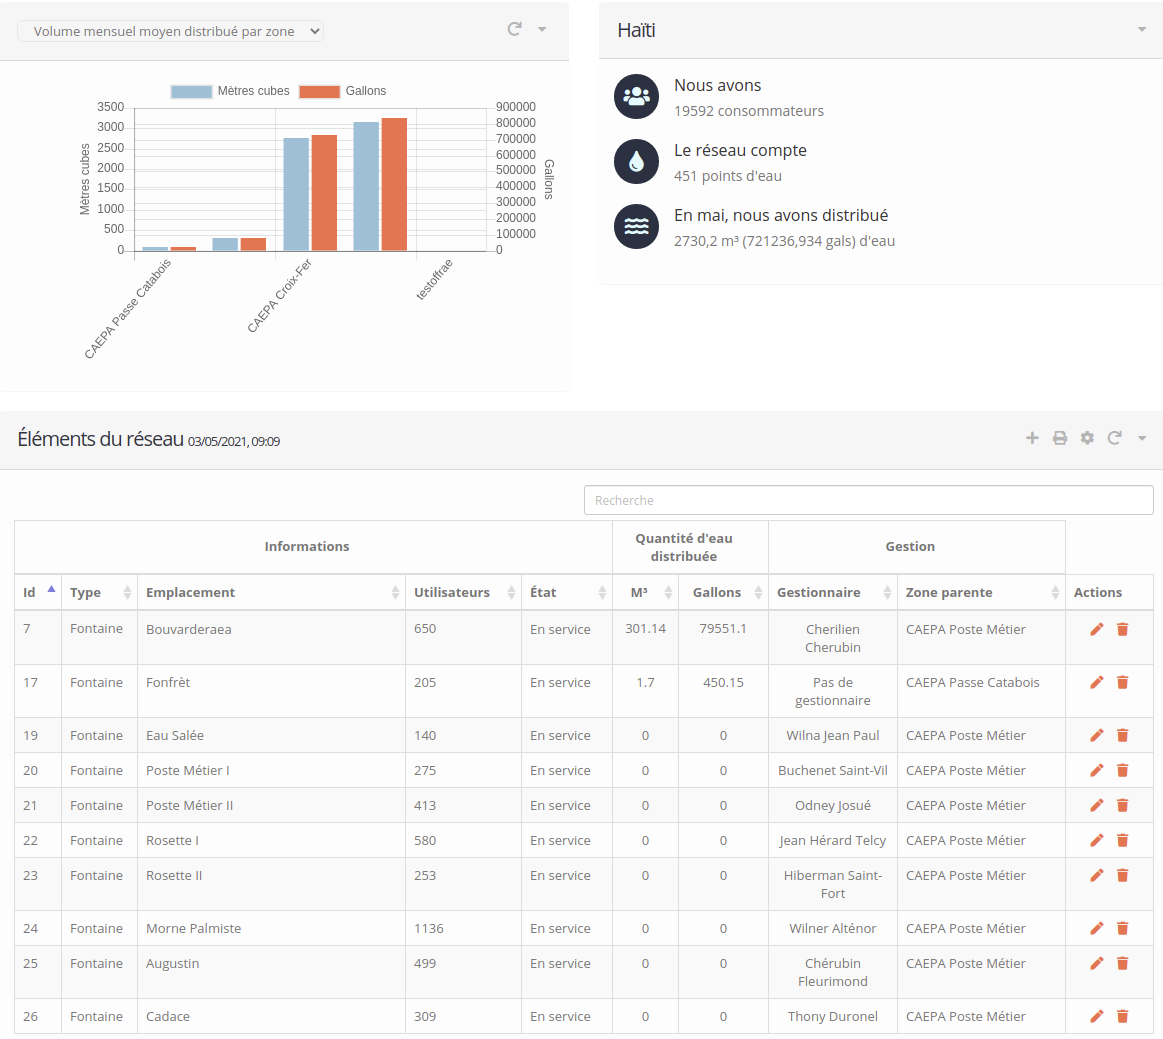
\includegraphics[width=1\textwidth]{images/water_elem}
					\caption{Module réseau}
				\end{figure}
				
\newpage
				
			\subsection{Carte}
				Ce module comprend un tableau réduit des éléments du réseau ainsi qu'une carte interactive qui permet à l'utilisateur de voir où sont situés les différents éléments du réseau et de connaître ou d'encoder les coordonnées géographiques de ceux-ci. Pour encoder ces coordonnées, l'utilisateur peut soit les entrer manuellement soit utiliser la carte intéractive prévue à cet effet. 
			
			Comme dans le module décrit au point \ref{sec:reseau}, l'utilisateur peut ajouter, supprimer ou modifier des éléments du réseau dans ce module.
			
				\begin{figure}[H]
					\centering
					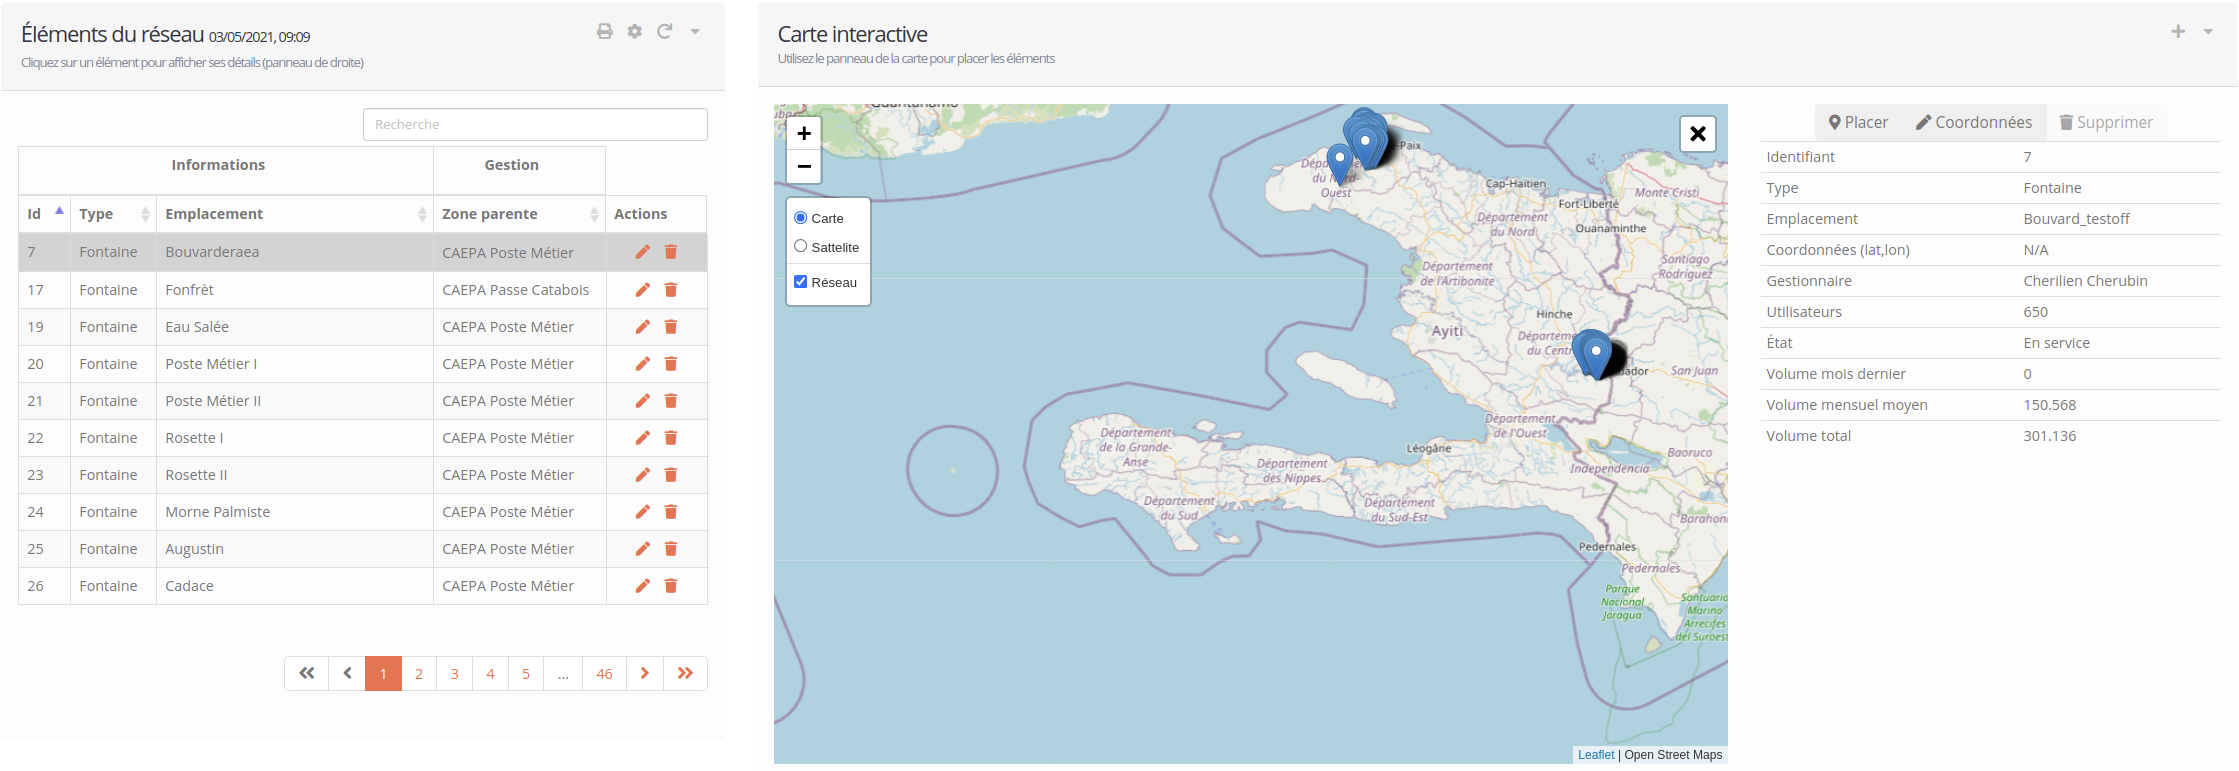
\includegraphics[width=1\textwidth]{images/map}
					\caption{Mordule carte}
				\end{figure}
				
				\begin{figure}[H]
					\begin{subfigure}[b]{0.5\textwidth}
  						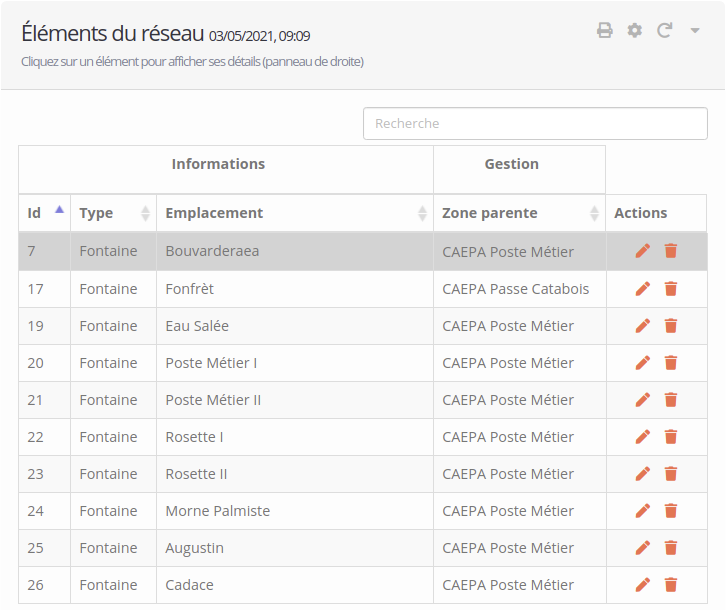
\includegraphics[width=1\linewidth]{images/map_tab1}
  						\caption{Tableau des éléments réseaux simplifié}
					\end{subfigure}%
					\begin{subfigure}[b]{0.5\textwidth}
  						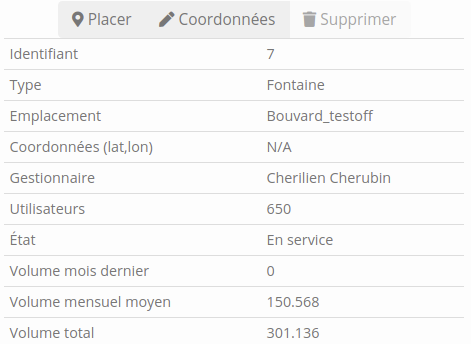
\includegraphics[width=1\linewidth]{images/map_tab2}
  						\caption{Détails de l'élément réseau}
					\end{subfigure}
					\label{fig:test}
				\end{figure}
				
			\subsection{Gestion de zone}
				Ce module comprend 3 tableaux permettant à l'utilisateur de gérer la zone qui lui est attribuée.
				\begin{description}
					\item[Zones] Le premier contient les différentes zones géographiques encodées dans le système. Cliquer sur un des éléments du tableau permet de filtrer les éléments des deux autres tableaux qui seront décrits plus bas afin de ne garder que les éléments de la zone concernée. Ce tableau permet également si l'utilisateur a les privilèges requis d'ajouter, de supprimer ou de modifier une zone.
					\item[Gestionnaires] Le deuxième contient la liste de tous les gestionnaires. Cliquer sur un gestionnaire permet à l'utilisateur de filtrer les éléments réseaux qui sont gérés par ce gestionnaire. De nouveau si l'utilisateur possède les privilèges nécessaires, il pourra ajouter, modifier ou supprimer des gestionnaires.
					\item [Elements du réseau] Le dernier contient le même tableau que dans la section \ref{sec:reseau}.
				\end{description}
				\begin{figure}[H]
					\centering
					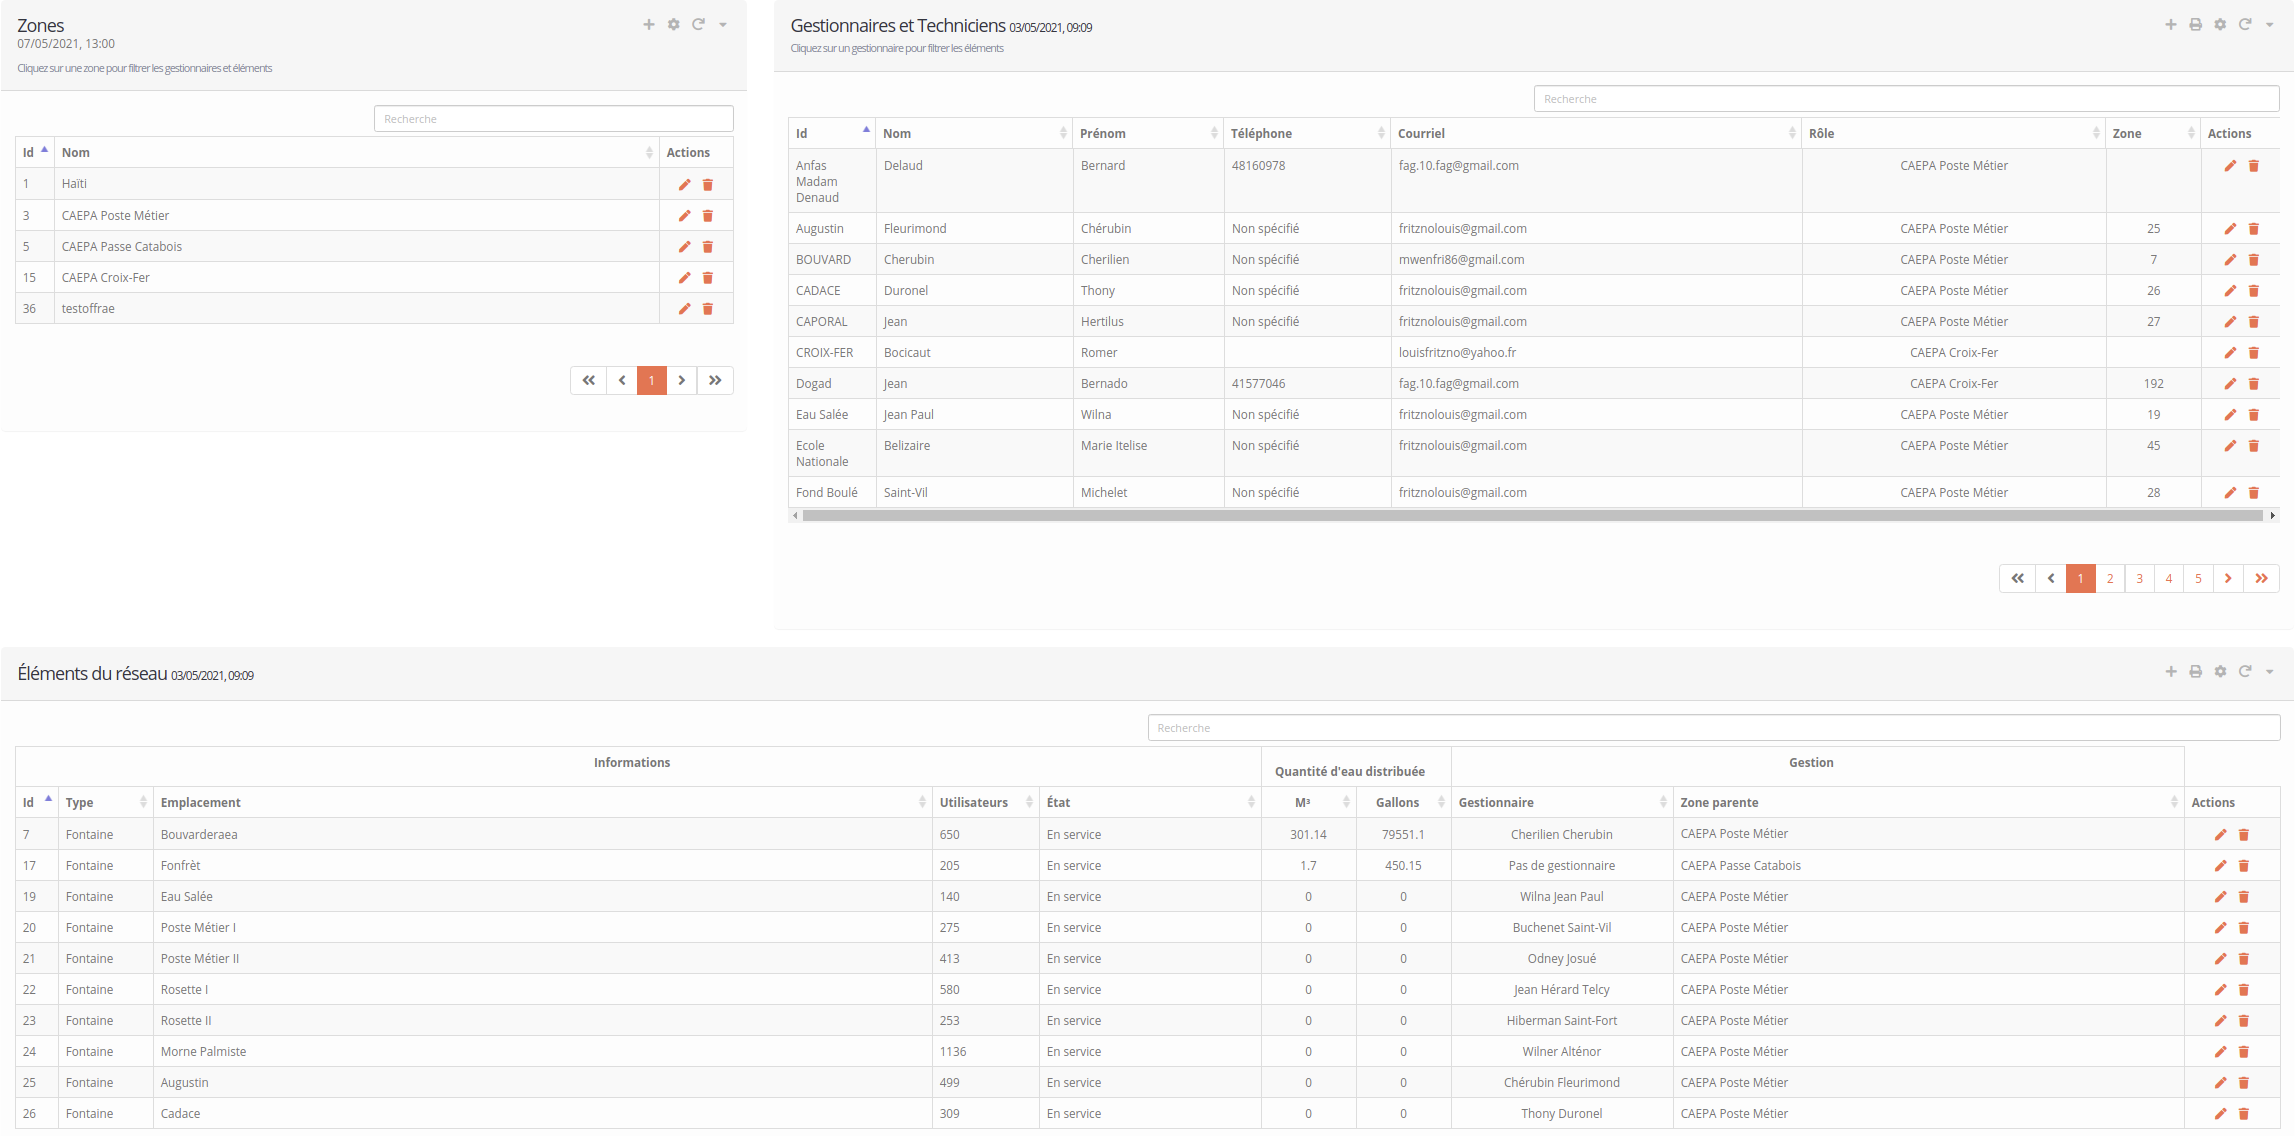
\includegraphics[width=1\textwidth]{images/gestion}
					\caption{Module gestion de zone}
				\end{figure}
			
				
				\begin{figure}[H]
					\begin{subfigure}[b]{0.3\textwidth}
  						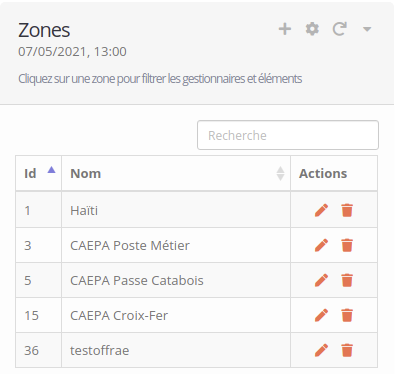
\includegraphics[width=1\linewidth]{images/gestion_tab1}
  						\caption{Tableau des zones}
					\end{subfigure}%
					\begin{subfigure}[b]{0.7\textwidth}
  						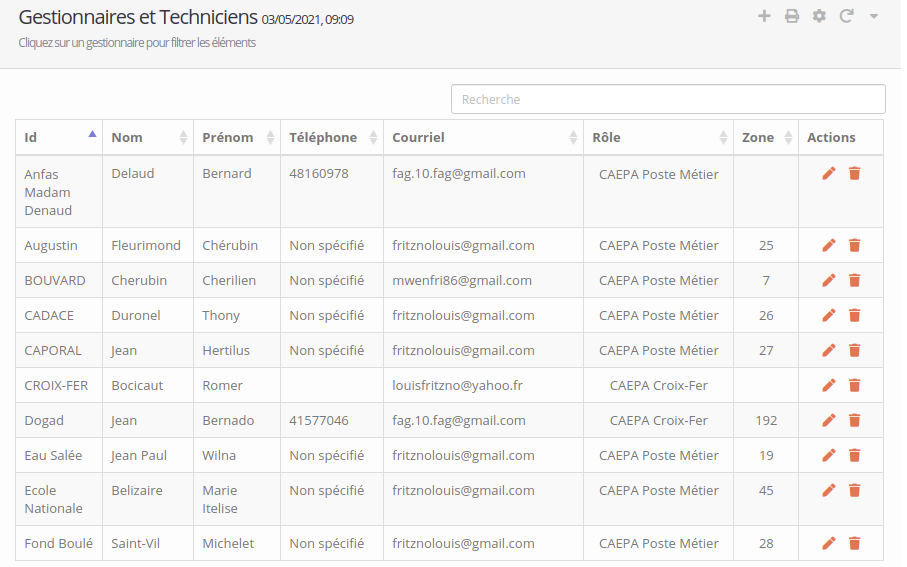
\includegraphics[width=1\linewidth]{images/gestion_tab2}
  						\caption{Tableau des gestionnaires}
					\end{subfigure}
					\label{fig:test}
				\end{figure}
			
			\subsection{Historique}
			\label{sec:historique}
				Ce module contient les actions ayant été effectuées par des gestionnaires de fontaines. Ces actions doivent être validées ou refusées par un gestionnaire plus haut placé. On peut y retrouver deux tableaux.
				\begin{description}
					\item[A valider] Ce tableau contient les éléments devant être validés. Ici si l'utilisateur a les privilèges requis, il peut choisir de confirmer ou non une action qui a été encodée.
					\item[Historique] Ce tableau contient les éléments qui ont été validés ou refusés dans les 3 dernières semaines. Il s'agit de l'historique récent des dernières modifications.
				\end{description}
				\begin{figure}[H]
					\centering
					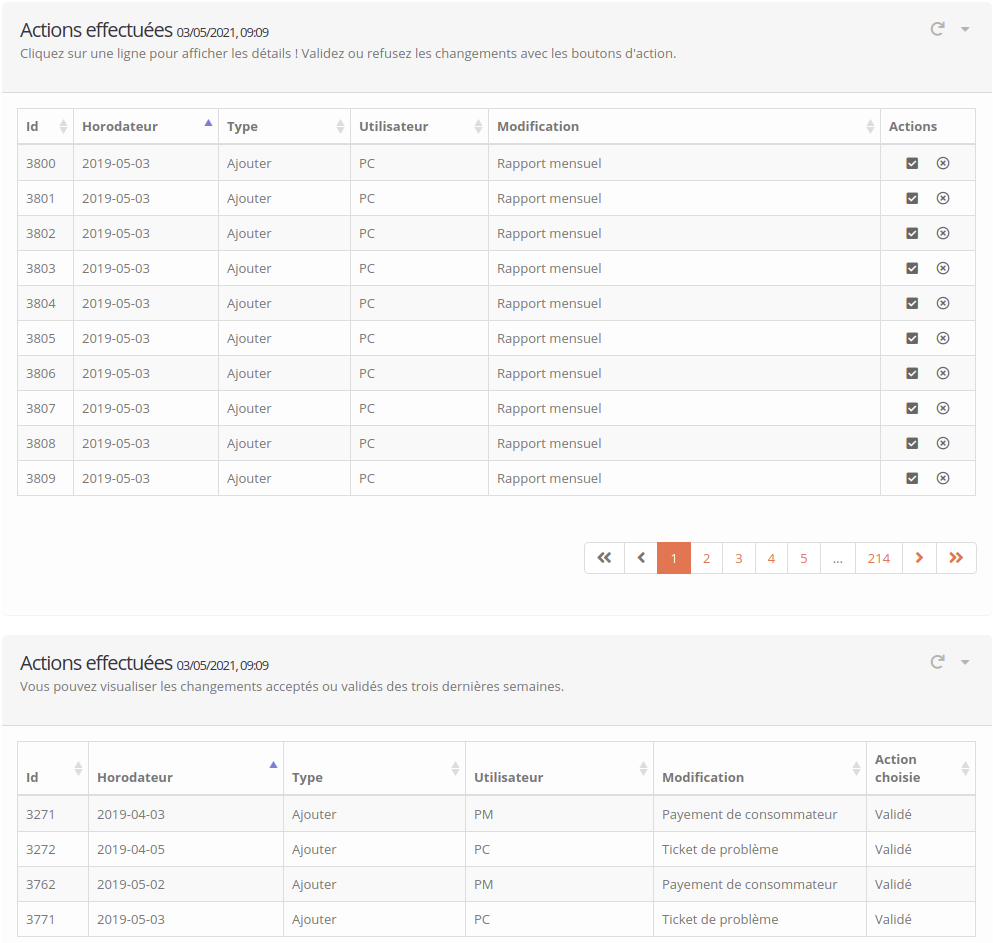
\includegraphics[width=1\textwidth]{images/logs}
					\caption{Module historique}
				\end{figure}
			
			\subsection{Rapports}
				Dans ce module, l'utilisateur peut signaler les différents problèmes qu'il rencontre avec les infrastructures de distribution d'eau potable. Une fois le problème signalé, celui-ci peut consulter ce qu'il a encodé dans le tableau juste en dessous et modifier ou supprimer son signalement. Si ses privilèges sont suffisamment élevés, il pourra également gérer les signalements d'autres personnes.
				
				C'est également ici que l'utilisateur va pouvoir encoder les rapports mensuels. Si jamais la connexion au serveur n'est pas disponible, il peut simplement enregistrer le formulaire avec les données qu'il a encodés afin de l'envoyer plus tard lorsque la connexion sera revenue.
				
				\begin{figure}[H]
					\centering
					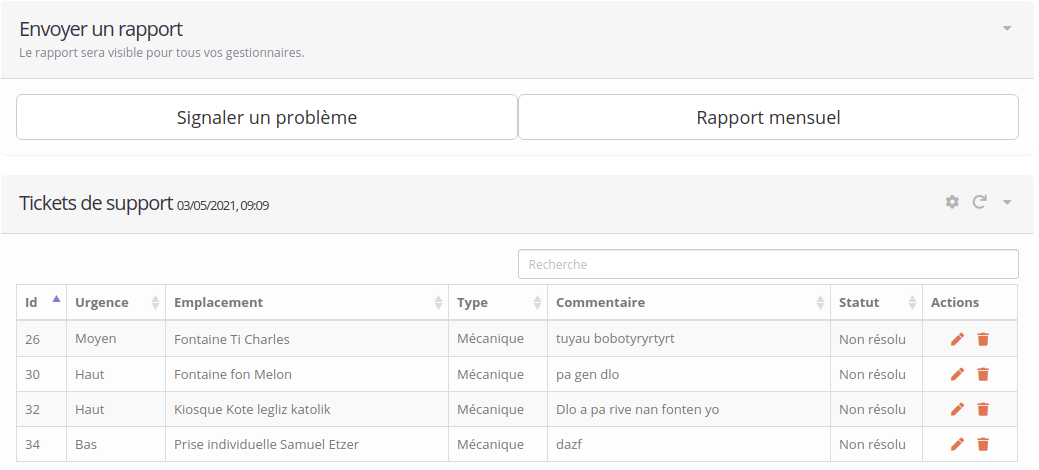
\includegraphics[width=1\textwidth]{images/report}
					\caption{Module rapport}
				\end{figure}
			
			\subsection{Consommateurs}
				Dans ce module, l'utilisateur retrouve 3 parties différentes :
				\begin{description}
					\item[Schéma] Le même choix de schéma que décrit dans la section \ref{sec:reseau}.
					\item[Résumé de zone] Un résumé de la situation  de la zone attibué à l'utilisateur (nombre de foyers consommant de l'eau, nombre de consommateurs, nombre de foyers n'ayant pas payé leur facture).
					\item[Consommateurs] Un tableau qui reprend tous les consommateurs auxquels l'utilisateur a accès. Celui-ci peut ajouter, modifier ou supprimer des consommateurs. Il peut également juste consulter tous les détails sur ceux-ci.
				\end{description}

				
				\begin{figure}[H]
					\centering
					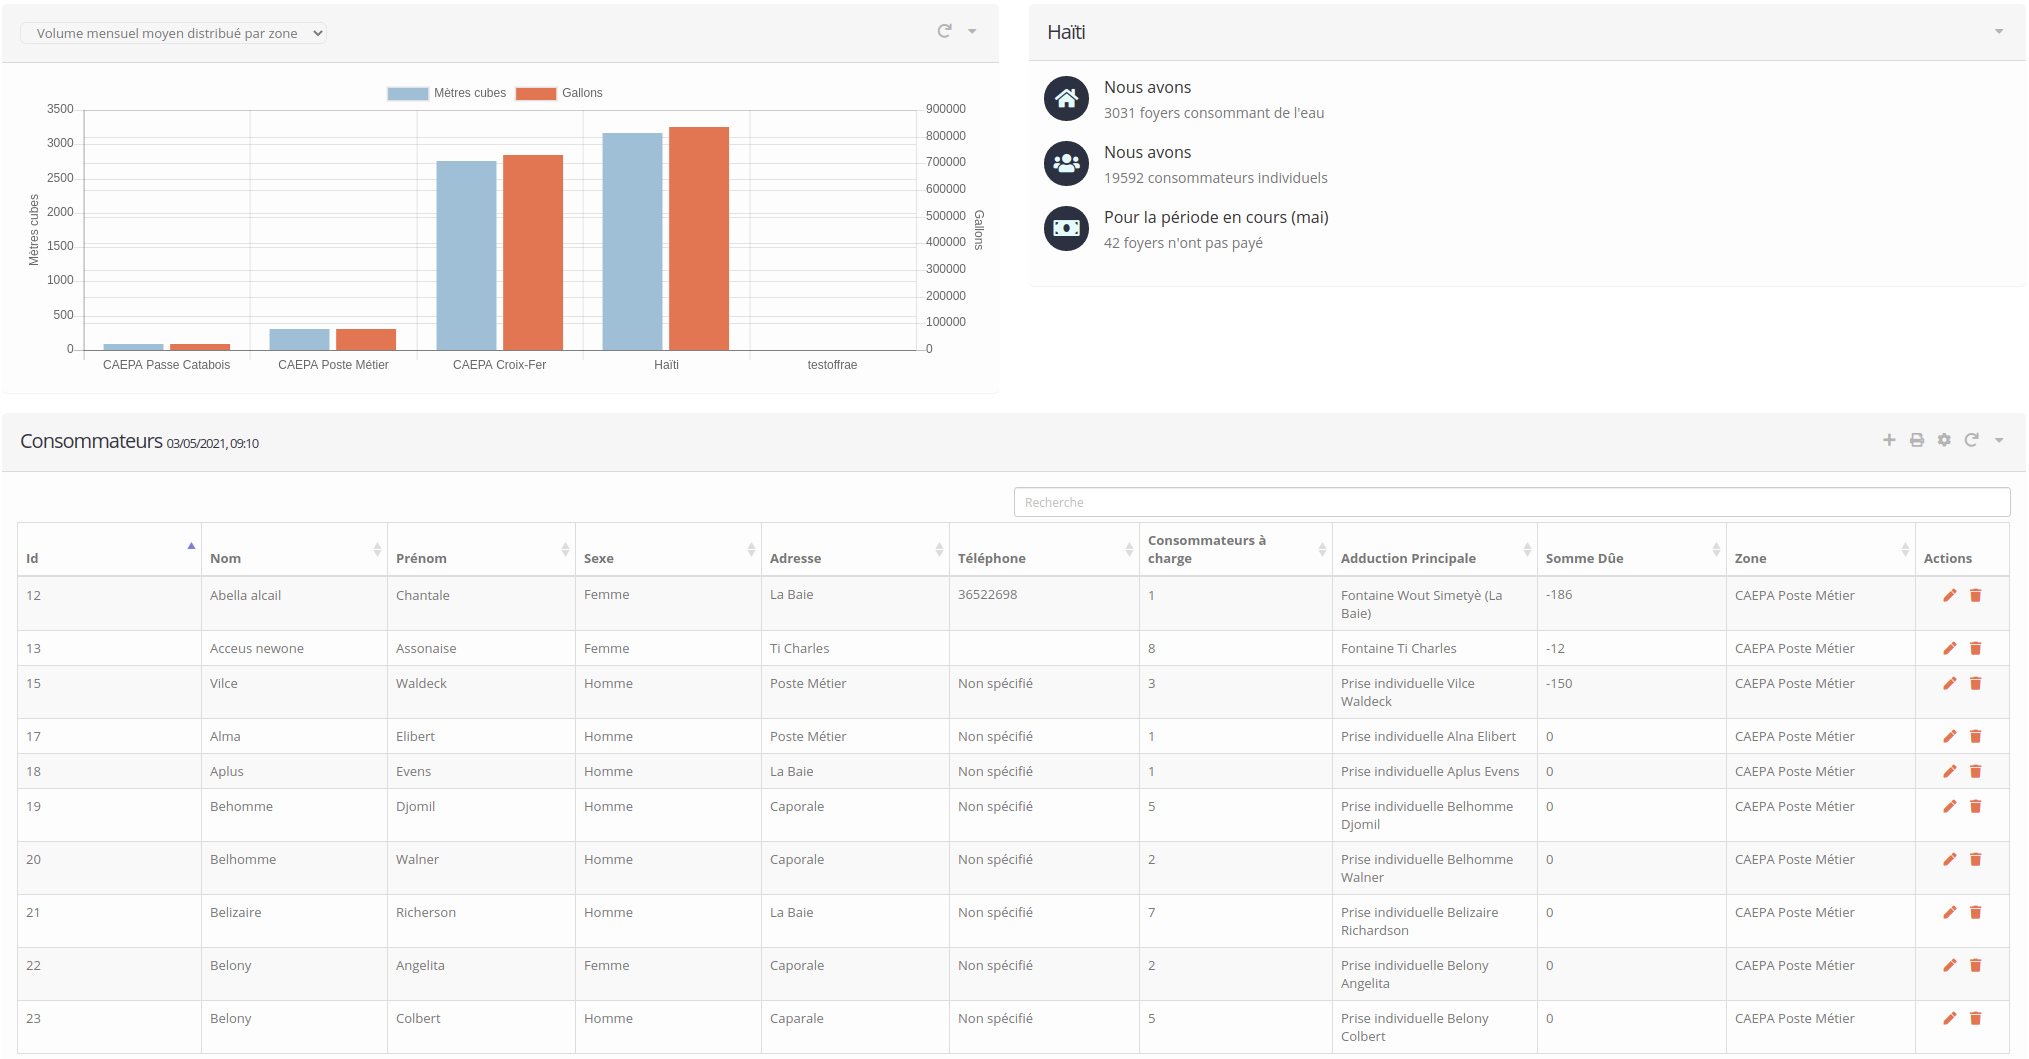
\includegraphics[width=1\textwidth]{images/consumer}
					\caption{Module consommateurs}
				\end{figure}
				
				\begin{figure}[H]
					\centering
					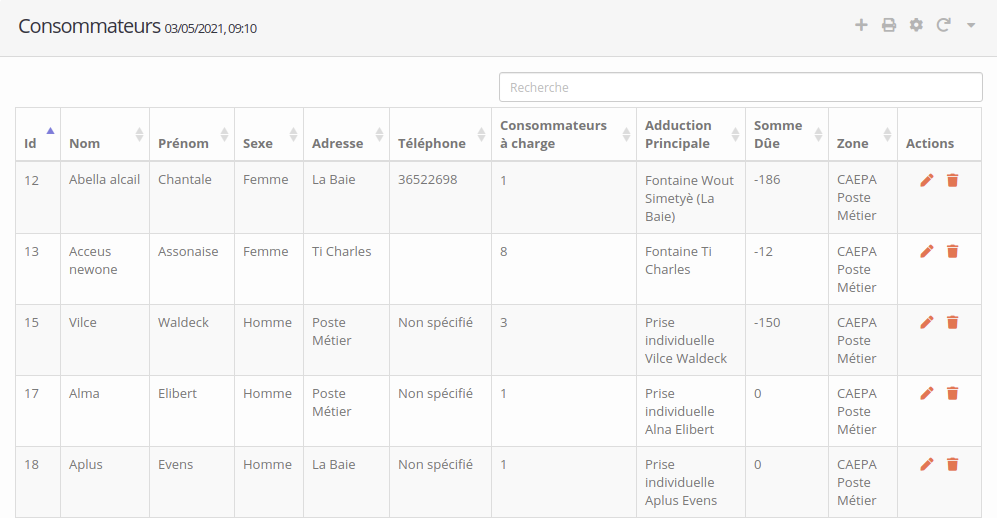
\includegraphics[width=1\textwidth]{images/consumer_tab1}
					\caption{Tableau des consommateurs}
				\end{figure}
			
\newpage
			\subsection{Finances}
				Dans ce module, l'utilisateur a accès à 4 tableaux différents qui lui permettent de gérer les finances de ses consommateurs. Celui-ci pourra modifier, supprimer ou ajouter des informations dans les différents tableaux en fonction de son niveau de privilèges.
				\begin{description}
					\item[Zones] Un tableau contenant les différentes zones. Le fait de sélectionner une zone permet à l'utilisateur de filtrer les consommateurs en fonction de leur zone d'attribution.
					\item[Consommateurs] Un tableau contenant les consommateurs auxquels l'utilisateur a accès. Le fait de sélectionner un consommateur permet de faire apparaître les deux tableaux suivants.
					\item[Détails] Un tableau contenant les coordonnées du consommateur sélectionné ainsi que la somme due par celui-ci. Il n'est pas possible de modifier des données manuellement dans ce tableau.
					\item[Paiements] Un tableau interactif contenant tous les paiements effectués par le consommateur sélectionné. Ici l'utilisateur peut ajouter, modifier ou supprimer des paiements du consommateur séléctionné.
				\end{description}
				
				\begin{figure}[H]
					\centering
					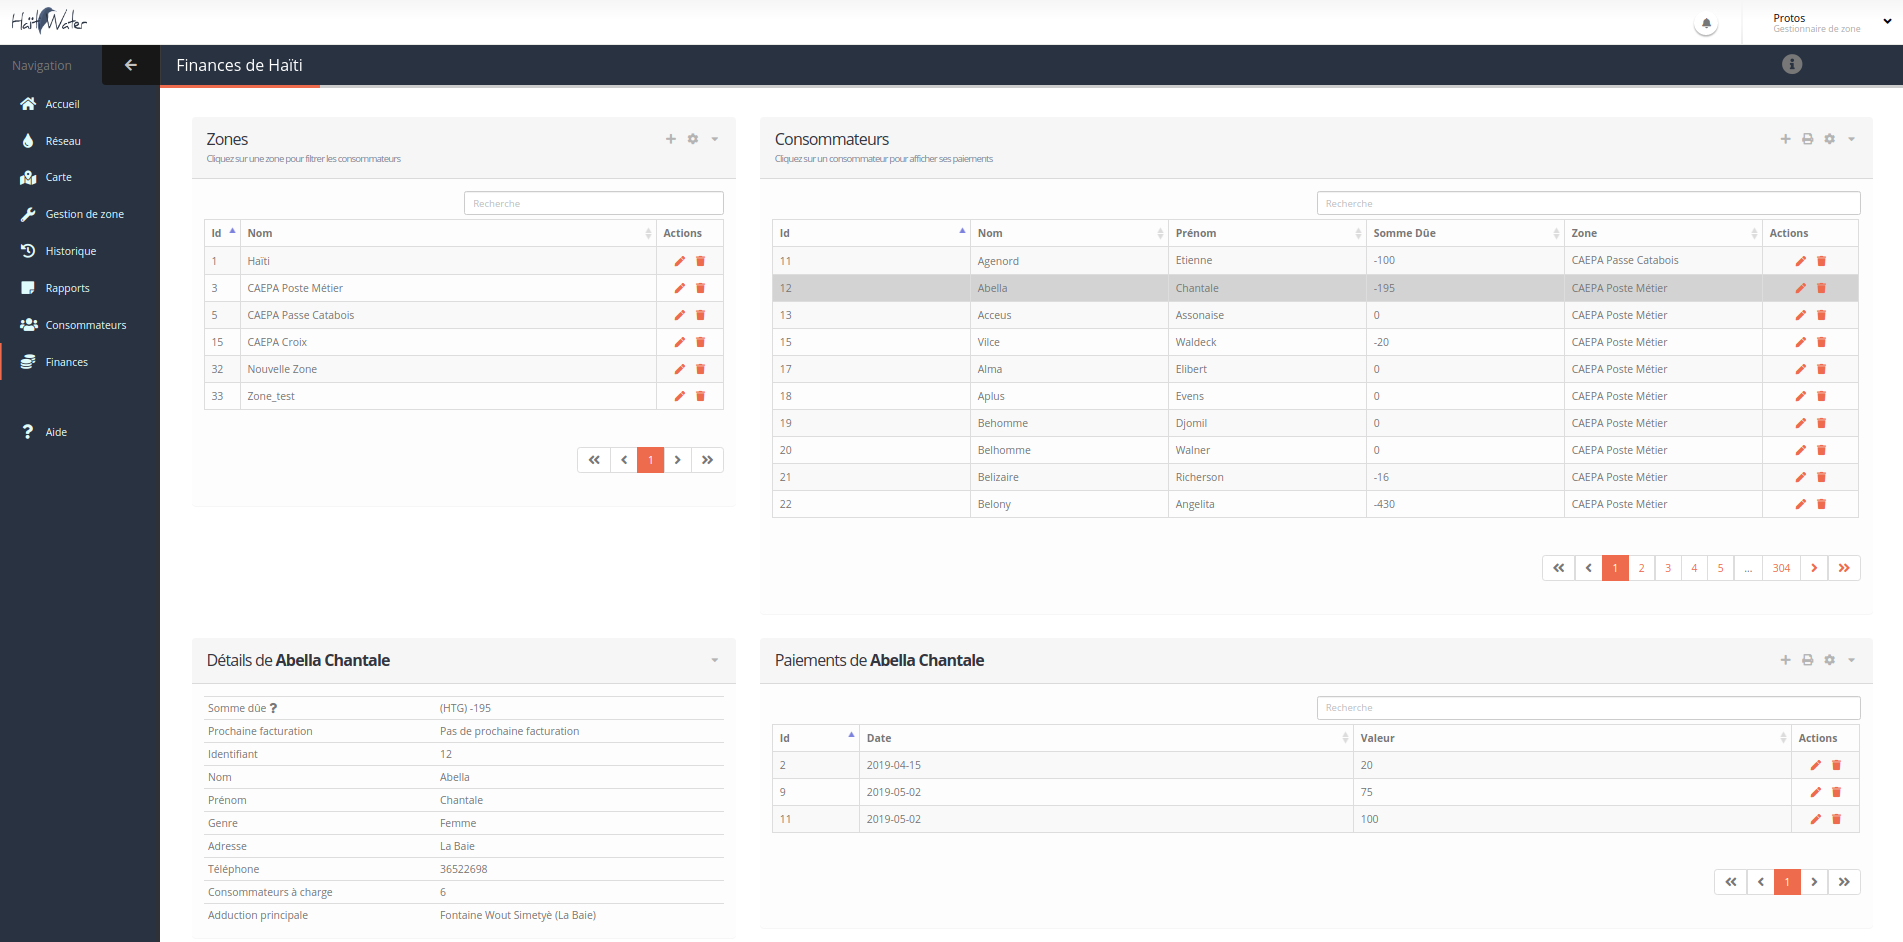
\includegraphics[width=1\textwidth]{images/finances}
					\caption{Module finances}
				\end{figure}
				
				
		\section{Problèmes réseaux}
			L'application HaïtiWater est une application web classique. Cela signifie que pour fonctionner, il faut qu'il y ait nécessairement une connexion à internet. Or en Haïti, cette connexion n'est pas très stable en ville et celui-ci peut aller jusqu'à être inexistant lorsque vous vous aventurez dans les zones les plus rurales. 
			
			Ces problèmes de connexions font que l'application est difficilement utilisable sur le terrain en toute sérénité car on ne sait jamais quand le réseau va devenir capricieux. Pour pallier ce problème, il a été décidé de faire évoluer l'application web existante pour que celle-ci puisse fonctionner même lorsque le réseau est absent.
				
			De par sa nature, une application web nécessite un connexion pour pouvoir fonctionner. Il a donc fallu étudier les différentes options qui pourraient permettre de faire fonctionner l'application hors-ligne. Parmis ces options,  les deux qui ont été retenues étaient de soit créer une \textbf{application mobile} séparée de l'application web, soit de transformer l'application web existante en \textbf{Progressive Web App}. 
				
			L'avantage de créer une application dédiée aux mobiles est qu'il est très simple de gérer le fonctionnement hors-ligne de cette application. De plus on peut plus facilement utiliser les différentes capacités de l'appareil mobile comme la caméra, la localisation, ...
			L'inconvénient de cette solution est qu'il faut du coup générer une nouvelle application de A à Z. De plus cela impliquerais deux codes sources différents à devoir maintenir.
				
			L'avantage de la Progressive Web App est que tout se joue au niveau du navigateur. Il n'est donc pas nécessaire de devoir maintenir un deuxième code source. De plus aucune installation n'est nécessaire de la part de l'utilisateur et les mises à jour de l'application sont faites de manière transparente.
			L'inconvénient de cette solution est que la gestion du mode hors-ligne est un peu plus complexe, on ne peut pas profiter des capacités de l'appareil mobile aussi bien qu'avec une application native et cette technologie étant assez récente, il n'y a pas énormément de ressources d'aide en ligne et tous les navigateurs ne prennent pas en charge toutes les fonctionnalités proposées.
				
		
			
			
%------------------------------------------------------------------------------------------

	\chapter{Organisation}
		Étant le seul étudiant à réaliser ce mémoire, il n'a pas été nécessaire d'utiliser des outils de planification complets. Cette section contiendra surtout la planification des différentes tâches à accomplir permettant l'aboutissement de l'application ainsi que l'écriture de ce mémoire. Celles-ci ont été mises en place grâce aux discussions avec mes deux promoteurs. 

		\section{Approche de travail}
			La première étape du mémoire a été de bien mettre en avant les différentes fonctionnalités à implémenter afin d'ajouter de la plus value au projet existant. L'idée de base étant de rendre l'application fonctionnelle hors-connexion.	
			
			Nous avons étudié la question avec mes deux promoteurs et Nahomie, l'étudiante venue d'Haïti. Celle-ci à pu nous apporter son expertise afin de séléctionner les fonctionnalités qui pourraient apporter une réelle valeur au projet et prioriser l'implémentation de celles-ci.
		
			%Comprendre les enjeux et les différentes problématiques a été la première tâche à accomplir. Il a fallut décider du type de technologie à utiliser afin d'apporter les fonctionnalités nécessaires au bon fonctionnement de l'application. 
			
			%La meilleure option aurait été de pouvoir en discuter avec la plupart des acteurs en Haïti afin d'avoir le plus d'avis possible sur la question. Mais vu le temps que cela aurait pris cette option n'était pas du tout envisageable. Pour pallier à se problème, nous avons étudié la question avec mes deux promoteurs et Nahomie l'étudiante venue d'Haïti. Celle-ci à pu nous apporter son expertise afin de choisir l'option idéale.
			
			%Une fois le choix technologique fait, nous avons effectuer la planification des tâches.
		
		

			%Etude du problème
			%Prioritisation des taches

			\subsection*{Planification}
				\label{sec:planification}
				
				\paragraph*{Mensuel}
				Dans un premier temps, il a fallu réaliser un plan général de déroulement du mémoire et mettre en avant les modules sur lesquels il fallait travailler en priorité et les différentes fonctionnalités à implémenter dans ceux-ci. Une grosse échéance était de pouvoir faire tester l'application par de vraie personne à partir de Février afin d'obtenir du feedback sur l'application.
				
				%Malgrè tout il était difficile de mettre des dates fixes car la technologie utilisée comporte encore peu de communauté et il est donc difficile de trouver des solutions "clé sur porte". 
				%La grande échéance posée était de pouvoir effectuer les tests de l'application avec des personnes réelles à partir de février afin d'avoir le temps de prendre compte les feedback pour améliorer l'application.
				
				\paragraph*{Hebdomadaire} 
				Une réunion était prévue toutes les semaines en alternance avec mes deux promoteurs. Ces réunions permettaient de leur montrer l'état d'avancement du développement et d'avoir un feedback extérieur sur celui-ci. Elles ont toutes eu lieu en vocal via l'application Teams. En effet en période de COVID, il était impossible de se voir régulièrement en présentiel.
				
				\paragraph*{Quotidien}
				Etant donné que j'étais le seul à travailler sur le mémoire, un outil de suivi n'était pas nécessaire. Pour gérer l'organisation du travail une simple liste de tâches était maintenue. Cette liste était modifiée tous les jours en fonction de l'avancement de celle-ci. Les plus importantes étaient maintenues en haut de la liste afin de les prioriser. 
				
				Le plan n'a malheureusement pas pu être entièrement respecté pour différentes raisons:
				\begin{itemize}
					\item La technologie étant encore assez récente, les sources d'informations et d'aides sur le net sont encore peu présentes. Du retard a donc été pris lors du développement de certaines fonctionnalités complexes.
					\item L'installation du serveur en Haïti a pris plus de temps que prévu et il a donc fallu repousser la validation avec de vraies personnes. 
					\item La période COVID-19 a apporté un manque de stimulation et de motivation qui a ralenti l'avancement du projet.
				
				\end{itemize}				
				
				Malgré le retard pris, il a tout de même été possible de terminer le projet dans les temps.
				
				
		\section{Méthodologie}
			Même en travaillant seul, une bonne méthodologie de travail permet de garantir l'avancement régulier du projet. Elle permettra de transformer efficacement les différents besoins en fonctionnalités implémentées.
			

			\subsection*{Agile}
				Le méthodologie agile permet une réponse au changement plus flexible. Plûtot que de planifier tout le projet directement, on développe par petit incrément que l'on termine à chaque itération. 
				
				Cette méthode a permis de faire évoluer le projet en fonction des différents feedback que j'ai reçu de la part de mes promoteurs et de l'étudiante venue d'Haïti. Ce qui n'aurait pas été possible avec une approche waterfall beaucoup plus séquentielle.
				
				\paragraph*{Feature Driven Development.} L'application a été développée avec la méthode de développement par les fonctionnalités. Dans cette méthode on se focalise surtout sur la création d'une liste de fonctionnalités et sur leurs productions. Ces différentes fonctionnalités ont été déterminées par mes deux promoteurs et l'étudiante Haïtienne.
				
				\paragraph*{Itérations.} Dans le cadre d'une méthodologie agile, les itérations sont de courtes durées. Lors de ce mémoire, les itérations duraient deux semaines. Cela permettait d'avoir un feedback de la part des deux promoteurs que je voyais en alternance une semaine sur deux. Les avantages des itérations courtes sont que l'on peut détecter rapidement les défauts présents et les corriger rapidement. 


			\subsection*{Phases du mémoire}
		
			
			\begin{figure}[H]
					\centering
					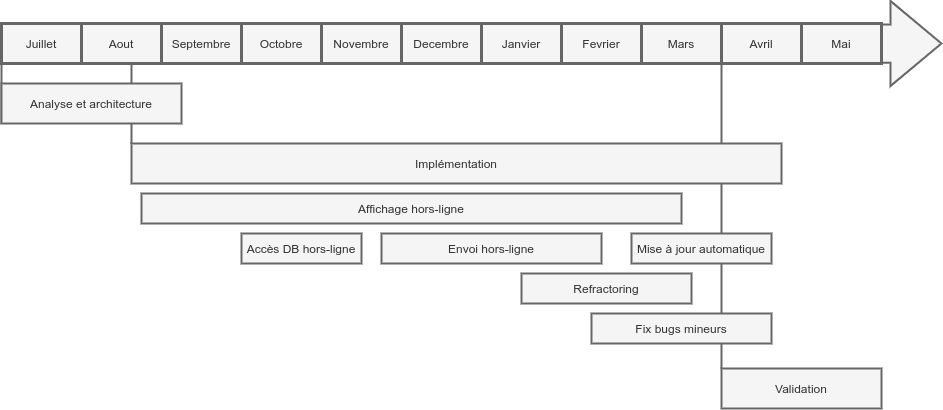
\includegraphics[width=1\textwidth]{images/Gantt}
					\caption{Diagramme de Gantt}
					\label{fig:Gantt}
				\end{figure}
				
			\paragraph*{Analyse et architecture.}
			Sur le schéma \ref{fig:Gantt}, on peut voir qu'il y a d'abord une phase d'analyse afin de déterminer les technologies qui seraient utilisées pour les différentes fonctions à implémenter. C'est dans cette phase qu'il y a eu beaucoup de discussions avec l'étudiante venue d'Haïti.
		
			\paragraph*{Implémentation.} 
			Cette phase compose la plus grosse partie du mémoire. C'est ici que toutes les décisions prises durant la phase d'analyse se sont mise en place. Cette phase se divise en plusieurs petites phases qui représentent les différentes fonctionnalités produites durant le mémoire. 
			
			\paragraph*{Validation.}
			La phase de validation n'intervient que tard dans le déroulement du mémoire. C'est simplement parce que la méconnaissance de la technologie à utiliser et le temps qu'a pris le déploiement de l'application sur les serveurs Haïtiens ont grandement retardé l'arrivée de cette phase.			
			
			\paragraph*{Rédaction.}
			La rédaction du mémoire n'a commencé que lorsque la plupart des fonctionnalités étaient terminées afin de lancer la validation au plus vite. Durant la rédaction, les parties produites ont été relues par mes deux promoteurs séparément afin d'améliorer celle-ci mais aussi par des relecteurs externes afin que le texte soit plus agréable à lire. 
			
			
			
			
			
%---------------------------------------------------------------------------------------------

	\chapter{Analyse des besoins}
		\label{sec:analyse_besoins}
		Cette phase est très importante. C'est lors de celle-ci que nous, mes deux promoteurs, l'étudiante d'Haïti et moi-même, avons choisi quelle technologie était la plus adaptée afin de faire évoluer l'application existante de la meilleure façon possible. C'est également ici qu'ont été déterminées toutes les fonctionnalités à implémenter et leur ordre de priorité.
		
		J'ai avec l'aide de l'étudiante Haïtienne et les bons conseils de mes promoteurs, realisé une analyse de Moscow qui sera décrite dans la section \ref{sec:besoins_fonctionnels}. Cette méthode permet de prioriser les tâches d'un projet en fonction de leur criticité, c'est-à-dire du niveau d'impact de la tâche sur la réalisation du projet.
		Cette analyse de Moscow est assez représentative de la direction que devait prendre le projet et représente bien les différentes tâches à accomplir.


		\section{Besoins fonctionnels}
			\label{sec:besoins_fonctionnels}	
				
			\begin{figure}[H]
				\centering
				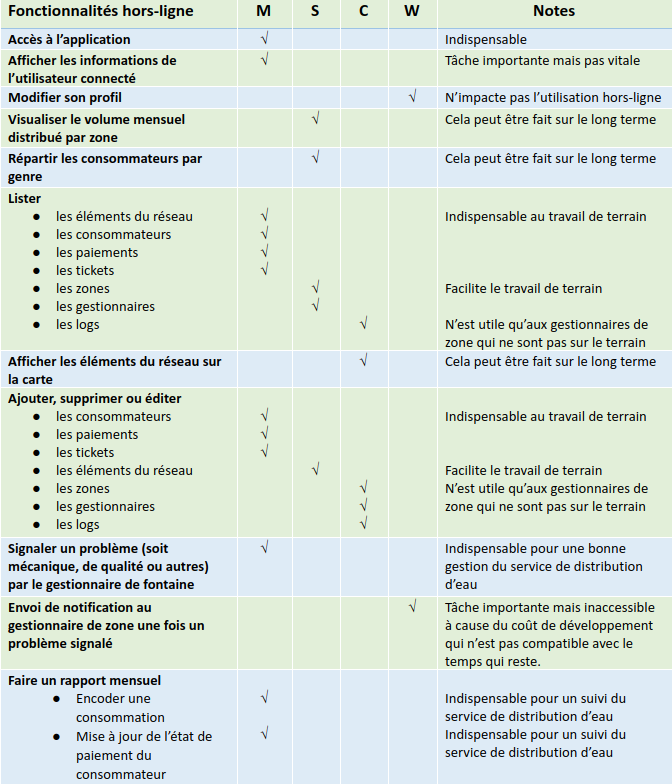
\includegraphics[width=1\textwidth]{images/moscow}
				\caption{Moscow}
				\label{fig:moscow}
			\end{figure}
			
			Les besoins fonctionnels répondent aux points précis à implémenter, ils représentent toutes les tâches à accomplir pour que le projet soit réussi. Dans le tableau \ref{fig:moscow}, les lettres ont le signification suivante: 
			\begin{description}
				\item[M] signifie "Must have", le projet serait un échec si l'application ne possèdait pas cette fonctionnalité à la fin du développement.
				\item[S] signifie "Should have", cette fonctionnalité doit être faite dans la mesure du possible. Ces tâches sont importantes mais pas vitales.
				\item[C] signifie "Could have", cette fonctionnalité peut être faite si cela n'affecte pas les autres tâches importantes. Ce sont des tâches de confort qui peuvent être effectuées si vous avez suffisamment de temps et que les tâches des deux catégories précédentes ont été réalisées.
				\item[W] signifie "Won't have but would like", ce qui ne sera pas fait cette fois, mais plus tard. Réaliser ces tâches est un luxe qu'on a théoriquement pas le temps de se payer.
			\end{description}
			
			Toutes les taĉhes de type \textbf{M}, \textbf{S} et \textbf{C} ont été réalisée durant ce projet. Seule les tâches \textbf{W} n'ont pas été implémentées.
			
			Lors de l'analyse des besoins, nous avons bien entendu repris l'analyse faite par les anciens mémorants \cite{ref:haitiwater}. Ils proposaient trois types différents d'accès à l'application et aux données lorsque le réseau n'est pas disponible. Les 3 options proposées sont les suivantes. 
			\begin{description}
				\item[Accès aux formulaires.] Avec cette solution, l'utilisateur aurait toujours un accès aux différents formulaires d'ajouts de données. Celui-ci pourrait pré-remplir les formulaires et les enregistrer dans le cache du navigateur afin de pouvoir les envoyer plus tard dans le cas où le réseau ne serait pas disponible immédiatement. Cette solution est déjà partiellement mise en place dans l'application de base. Il est en effet déjà possible de pré-remplir son rapport mensuel et de le sauvegarder pour plus tard. %C'est la solution la plus simple car elle ne demande pas d'avoir les données de la base synchronisées localement. Pourtant cette solution n'a pas été retenue car celle-ci est trop simpliste et ne permet pas une utilisation suffisante en cas de perte de connexion.
				\item[Accès statique aux données.] Cette solution demande d'avoir une version simplifiée de la base de données en copie sur l'appareil de l'utilisateur mais sans la possibilité de modifier celle-ci. Cela permettrait aux utilisateurs de consulter les données hors-ligne mais pas d'en entrer de nouvelles. L'avantage de cette solution est que la synchronisation des tables est très simple et qu'il n'y a pas de problèmes d'inconsistances des données qui peuvent arriver lorsque deux utilisateurs modifient la même donnée en étant hors-ligne.
				\item[Accès complet aux données.] Cette solution permettrait aux utilisateurs de pouvoir consulter, ajouter, supprimer et modifier des données de la base de données. Ainsi même en cas de perte de réseau, l'utilisateur pourrait continuer à réaliser ses tâches sans le moindre soucis. Cette solution est la plus compliquée à mettre en place car elle demande de synchroniser les différentes versions des données. En effet si deux utilisateurs modifient en même temps les mêmes données en étant hors-ligne, il faudrait pouvoir déterminer quelle modification conserver sans créer d'inconsistances.  
			\end{description}
			
			L'option qui a été choisie est celle de l'accès complet. C'est la seule solution qui permettrait vraiment à l'application d'être utilisée de manière intensive sur le terrain. C'est également l'option la plus intéressante à mettre en place du point de vue technique.
			
			
			
			\subsection*{Affichage des pages}
				Une partie importante des besoins est bien évidemment l'accès aux différentes pages de l'application lorsque la connexion internet n'est plus disponible. 
				
				C'était la partie prioritaire du projet car sans cette fonctionnalité, il aurait été impossible d'accèder aux différentes données. Les premières pages concernées par cette évolution ont été celles utiles aux gestionnaires de fontaines qui sont le plus souvent sur le terrain.
				Les différents points du tableau \ref{fig:moscow} concerné par cette partie sont :
				\begin{itemize}
					\item L'accès à l'application
					\item Afficher les informations de l'utilisateur connecté
					\item Visualiser le volume mensuel distribué par zone
					\item Répartir les consommateurs par genre
				\end{itemize}
				
				Comme on peut le voir les deux premiers points sont bien placés dans la catégorie "Must have". Les deux derniers sont dans le "Should have" car ces fonctionnalités ne sont que des schémas qui s'affichent sur certaines pages et ceux-ci ne sont pas absolument essentiels.
				
			\subsection*{Accès aux données}
				La deuxième partie importante des besoins fonctionnels est d'avoir accès aux données de la base de données même lorsque la connexion au serveur n'est pas disponible. En effet le simple accès aux pages hors ligne n'a que peu d'intérêt si l'on ne peut pas consulter de données sur ces pages.
			Dans le tableau \ref{fig:moscow}, cela est représenté les points suivants :
				\begin{itemize}
					\item Lister les éléments du réseau
					\item Lister les consommateurs
					\item Lister les paiements
					\item Lister les tickets
					\item Lister les zones
					\item Lister les gestionnaires
					\item Lister les logs
				\end{itemize}
				
				Les quatres premiers points sont dans la catégorie "Must have" car ceux-ci représentent les données qui seront utilisées en permanence par les acteurs sur le terrain, dans notre cas les gestionnaires de fontaines. Ce sont donc les données qu'il faut avoir prioritairement dans l'application hors-ligne.
				
				Les trois derniers sont dans la catégorie "Should have" et "Could have" car ceux-ci sont surtout utiles pour les gestionnaires de zones qui seront assez peu sur le terrain. Malgrè tout il reste intéressant de pouvoir accèder à ces données même lorsque la connexion au serveur n'est pas disponible dans le cas où un gestionnaire devrait se déplacer sur le terrain ou bien en cas de panne du réseau internet.
				
				Un dernier point non listé est d'afficher les éléments du réseau de distribution d'eau sur une carte interactive même lorsque l'on a pas de connexion réseau. Ce point a été mis dans les "Could have" car l'usage de la carte en mode hors-ligne est une fonction qui prendrait beaucoup d'espace sur un appareil mobile et cette fonctionnalité n'est pas essentielle à un usage sur le terrain.

			\subsection*{Modifications des données}
				\label{sec:gest_donnee}
				La dernière partie mais non la moindre consiste à gérer l'envoi des données lorsque la connexion au réseau n'est pas disponible. Cela permettrait aux utilisateurs de pouvoir complétement se passer de la solution crayon/papier.
				Dans le tableau \ref{fig:moscow} cette partie est représentée par les points suivant:
				\begin{itemize}
					\item Ajouter, supprimer ou éditer
					\begin{itemize}
						\item Les consommateurs
						\item Les paiements
						\item Les tickets
						\item Les zones
						\item Les gestionnaires
						\item Les logs
					\end{itemize}
					\item Signaler un problème par le gestionnaire de fontaine
					\item Faire un rapport mensuel
				\end{itemize}
				
				La plupart des points sont situés dans la partie "Must have" car ces fonctionnalités sont essentielles au bon fonctionnement de l'application hors-ligne. Par contre la modification des éléments du réseau, des zones, des gestionnaires et des tickets sont dans les catégories "Should have" and "Could have" car ces données sont surtout utilisées par les gesionnaires de zones qui ne vont que peu sur le terrain.			

		\section{Besoins non-fonctionnels}
			Les besoins non-fonctionnels sont soit des besoins optionnels, soit des besoins liés à l'implémentation et à l'interopérabilité générale. C'est en réalisant ces besoins non fonctionnels, que l'on obtient un système fiable et qualitatif.
					
			\subsection*{Multi-plateforme}
			\label{sec:multi}
				Ce projet se déroule dans le cadre, et est la suite, d'un mémoire universitaire. La prochaine étape pour celui-ci une fois le mémoire terminé est qu'il soit déployé et maintenu par une équipe de développeur en Haïti. 
				
				Le problème est qu'on ne connait pas encore le temps et le budget qui seront alloués à la suite de ce projet. Par contre, ce que l'on sait, c'est qu'il faut que l'application puisse tourner sur un maximum d'appareils différents. Les choix technologiques qui seront décris dans le section \ref{sec:choix_tech} ont donc été pris en prenant en considération le fait que l'application doit pouvoir tourner sur tout type de configuration.
				
			\subsection*{Technologies simples et populaires}
				Comme précisé précédemment, nous ne connaissons pas encore l'équipe de développeur qui va reprendre le projet. Il a donc fallu continuer à utiliser des technologies qui sont assez rapide à apprendre et accessible à tous. Cela afin de faciliter la maintenance et l'évolutivité de l'application lorsque celle-ci sera déployée en Haïti.	
				De plus il faudra également fournir une documentation complète et détaillée afin d'aider ces futurs développeurs lorsqu'ils devront reprendre l'application.
				
		\section{Structure des données hors-ligne}
			\label{sec:data}
			Pour que l'utilisateur puisse accèder aux données en étant hors-ligne, il faut bien évidemment que celles-ci soient stockées sur l'appareil. Pour ce faire il a fallu trouver une solution qui prendrait peu de place sur l'appareil de l'utilisateur, qui permettrait un accès rapide en lecture et la possibilité de modifier ces données. Deux solutions ont alors été envisagées.
			\begin{description}
				\item[JSON] Stocker les réponses au format JSON telles qu'envoyées par le serveur dans la cache du navigateur. L'avantage de cette solution est qu'il est très rapide de récupérer les données à afficher sur la page lors du chargement de celle-ci car les données nécéssaires sont stockées telles quelles dans le navigateur, elle est également très facile à mettre en place. Si l'on avait utilisé l'accès statique aux données comme décrit dans la section \ref{sec:besoins_fonctionnels}, cette solution aurait été suffisante. Mais comme il faut pouvoir modifier les données, cette solution n'est pas la plus adaptée car il faudrait mettre le json en mémoire, le modifier et ensuite réecrire tout le nouveau JSON dans le cache a chaque modification de données.
				\item[DB] Utiliser un système de gestion des données intégré au navigateur. Cette option a pour avantage le fait d'avoir un vrai système de gestion de données. Une fois les données enregistrées dans le navigateur, il est très facile de faire des requêtes sur ces données ou bien d'ajouter en modifier certaines. Par contre l'inconvénient est que lors de la synchronisation des différentes tables dans le navigateur, l'appareil doit fournir un travail supplémentaire.
			\end{description}
				
			La solution qui a été retenue est la deuxième option. C'est en effet elle qui permet le plus facilement de gérer l'accès complet à l'application en permettant de modifier, supprimer ou ajouter des données hors-ligne.
			
			
		\section{Conclusion}
			Dans ce chapitre, une analyse poussée des besoins fonctionnels et non fonctionnels a été faite afin de déterminer les différentes fonctionnalités à implémenter et leur ordre de priorité. Une étude des différentes options de synchronisation des données a également été réalisée afin de trouver la solution qui serait la plus adaptée à un usage de l'application sur le terrain en cas de perte de connexion au réseau internet.
			
			




%------------------------------------------------------------------------------------------------------------
	\chapter{Implémentation}

		\section{Application de base}
			Dans cette section, un résumé de l'application HaïtiWater créée précédemment vous sera présenté. Si vous désirez de plus amples informations sur les raisons des choix technologiques suivants et les détails de leur implémentation, vous pouvez consulter le document \cite{ref:haitiwater}.
			
			\subsection*{Backend}
				L'application HaïtiWater est une application web propulsée par le langage python. C'est ce langage qui a été choisi pour le backend car c'est un langage de programmation populaire et facile à apprendre. Il existe énormément de librairies logicielles et de documentations sur internet ce qui le rend plus facile à apprendre pour la future équipe développement. 
				
				Vu la taille du projet un framework a du être utilisé, l'organisation et la structure du framework permet une productivité plus élevée qu'un développement qui partirait de zéro et facilite la maintenance de l'application grâce une bonne organisation du code source. Le choix s'est porté sur Django principalement pour ses outils de gestion de base de données, particulièrement efficace pour les données géographiques.	
			
				Le SGBD utilisé pour l'application est PostGreSQL. Celui-ci a été choisi pour deux raisons :
				\begin{itemize}
					\item D'abord parce que c'est le système qui est recommandé par Django car c'est celui qui s'adapte le mieux à l'Object relational mapping. C'est Django qui va se charger d'effectuer la connexion avec la base de données et qui va se charger d'y envoyer toutes les requêtes.
					\item Ensuite parce qu'il existe l'extension PostGIS de PostGreSQL permettant de traiter facilement les données géographiques.
				\end{itemize}			
				
				Django utilise une architecture modulaire qui permet de faciliter l'évolution et la maintenance de l'application. la figure \ref{fig:modules} représente les relations entre les différents modules tels que présenté dans le mémoire de la première version de l'application \cite{ref:haitiwater}.
				
				\begin{figure}[H]
					\centering
					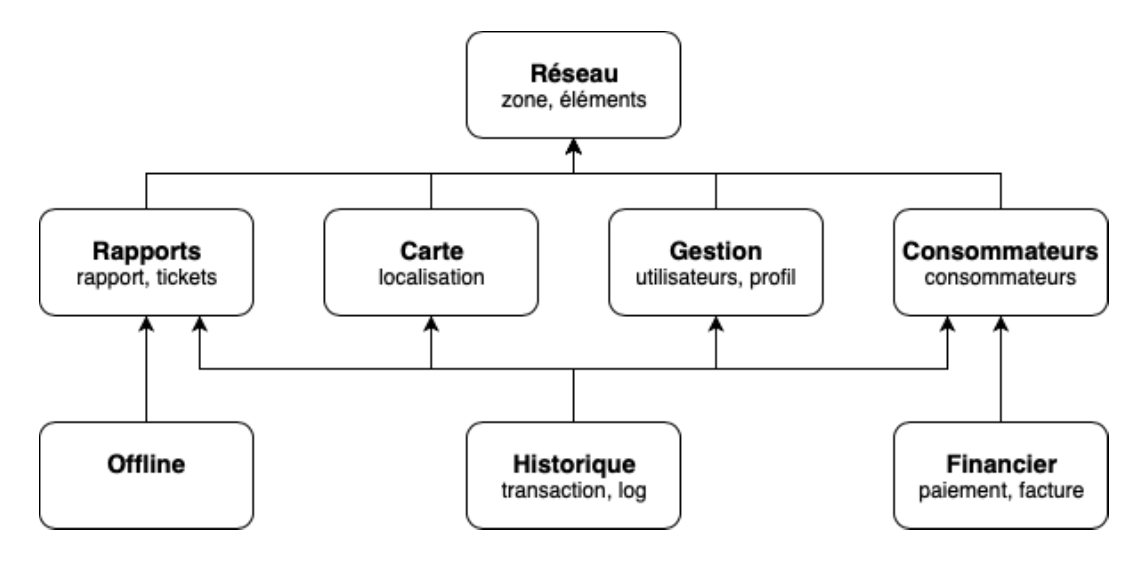
\includegraphics[width=1\textwidth]{images/modules}
					\caption{Relations entre les modules}
					\label{fig:modules}
				\end{figure}
							
				
				Le serveur possède également une API qui permet de séparer les différents rôles de celui-ci. Le rôle de cette API est de faire le lien entre l'ORM de Django et les requêtes du client pour récupérer des données dans la base de données. Les requêtes concernant une page à afficher et celle concernant les données sont donc séparées. Cela facilite la récupération des données par les différentes bibliothèques du frontend et permet en cas de création d'une autre application de continuer à récupérer les informations sur le serveur.
						
			\subsection*{Frontend}
				Pour le front-end, aucun framework n'a été utilisé mais seulement la librairie bootstrap qui permet d'agencer l'interface graphique par blocs et de les personnaliser. La raison de son utilisation et qu'il s'agit d'une bibliothèque très connue et utilisée et donc facile à apprendre.
				
				Deux autres bibliothèques ont été utilisées afin de gérer l'affichage des données dans l'application. La première est "datatable.js", cette bilbiothèque permet l'affichage des données sous forme de table. La deuxième est Chart.JS, elle permet l'affichage des données sous forme de graphiques. Toutes les données sont récupérées par les blibliothèques via l'API du serveur.
				
			\subsection*{Client}
				Du coté du client, l'application utilise la mise en cache afin d'éviter les télechargements répétitifs des mêmes fichiers. Pour gérer cette mise en cache, on fait ici usage du Service Worker qui se place en middleware entre le client et le serveur afin d'intercepter les requêtes pour les mettre en cache.

		
		\section{Choix technologiques}
			\label{sec:choix_tech}
			Une étude a été faite pour savoir qu'elle était l'option la plus adaptée pour que l'application puisse être accessible lorsque l'utilisateur n'a plus de connexion au réseau internet. Plusieurs options ont alors été envisagées.
			
			\subsection*{Application android}
				Cette option est la plus facile à implémenter pour gérer le fonctionnement hors-ligne de l'application. On aurait dans ce cas une application Android qui cohabiterait avec l'application web existante. Cela aurait permis aux gestionnaires de fontaines d'accèder à une version limitée de l'application sur leur téléphone ou tablette quand ils sont sur le terrain.
			
				Le problème de cette solution est qu'elle ne fonctionne que sur Android et pas sur les appareils Apple utilisant le système iOS. De plus elle oblige à maintenir et à faire évoluer deux codes sources dans deux langages différents ce qui demanderait plus de temps ou deux team de développement.
				
			\subsection*{Xamarin}
				Xamarin est une plateforme open source qui permet de créer des applications modernes et performantes pour android, iOS et Windows grace au .NET \cite{ref:xamarin}. Le gros avantage de cette solution est qu'il suffit d'utiliser la partie API existante du serveur pour pouvoir créer une application qui serait disponible sur tous types d'appareils.
			
				Le gros défault de Xamarin est qu'il faut un temps d'apprentissage avant utilisation. Cette technologie n'est pas ultra répandue et il sera donc plus difficile pour Haïti de faire maintenir et évoluer le projet. Même s'il s'agit d'une solution cross-plateforme, il faut tout de même écrire autant d'interface différentes que l'on a de plateforme cible. Dans notre cas Android, iOS et Windows
				
			\subsection*{React-native}
				Cette technologie permet d'écrire des applications qui seront disponible à la fois pour Android et iOS. Il est même possible de dériver facilement du React-native pour en faire une application web react. Cela permettrait de ne pas trop diversifier les codes sources et ainsi faciliter leur maintenance.
				
				La difficulté ici réside dans le fait que même si React-native permet de faire du cross-plateform, on va tout de même avoir besoin de connaître pertiellement le langage et les API native de la plateforme sur laquelle on crée l'application, ici iOS et Android. Bien que cette solution commence à être de plus en plus utilisée elle reste plus complexe à maintenir. De plus cette solution oblige tout de même à continuer de maintenir deux applications différents : l'application web et l'application React-native.
				
			\subsection*{Progressive web-app}
				Les Progressive web-app sont de simples applications web utilisants les nouvelles capacités des navigateurs modernes. Grâce aux service workers, l'application peut fonctionner lorsque la connexion au serveur n'est pas disponible et grâce à l'app-manifest, celle-ci devient "installable" sur un appareil mobile. Une fois installée, une progressive web-app peut tourner en plein écran pour faire croire qu'il s'agit d'une application native. Ce n'est bien sûr par réelement cas, l'appareil va simplement ouvrir une page du navigateur en plein écran pour donner l'illusion. 
				
				C'est cette solution qui a été choisie pour faire évoluer le projet. Les raisons de ce choix sont que :
				\begin{itemize}
					\item Il n'est pas nécessaire de devoir maintenir deux codes sources différents contrairement aux autres solutions citées précedemment.
					\item On peut entièrement réutiliser le code de l'application de base et l'améliorer.
					\item L'usage de service worker permet de diminuer la charge du serveur et d'améliorer l'expérience utilisateur sans que celui-ci ne doivent se soucier d'installer ou de mettre à jour l'application puisqu'il suffit de se connecter une fois à l'application pour que celle-ci s'installe automatquement.
				\end{itemize}
				
				
		\section{Client}
			Toute cette partie décrira la fonctionnement du service worker. Un service worker joue le rôle de serveur proxy entre une application web et le navigateur. C'est lui qui va permettre une utilisation de l'application déconnectée du réseau. Il va intercepter toutes les requêtes faites par le navigateur et va effectuer différentes actions en fonction de la requête interceptée. C'est via ce service worker que l'on accède aux nouvelles APIs des navigateurs \cite{ref:sw}.
			
			
			\subsection{Stratégie de synchronisation des pages}			
				Toutes les pages de l'application sont synchronisées à l'aide du service worker et sont stockées dans un des caches du navigateur. Les fichiers nécesaires à l'affichage des pages suivent différentes stratégies de synchronisation en fonction de leur usage.			
				
				\subsubsection*{Fichiers statiques}  
					Les feuilles de styles et les fichiers javascripts ne sont synchronisés qu'une seule fois lors de l'installation du service worker. Ceux-ci seront mis à jour à chaque fois que le service worker est remplacé dans le navigateur. Cela se produit lorsqu'une nouvelle version de celui-ci est disponible. 
					
					Si les développeurs veulent forcer la récupération de nouveaux fichiers, il leur suffit de changer la variable "cacheVersion" dans le code du service worker. Si jamais certains fichiers de styles ou certains fichier n'ont pas pu être téléchargés lors de l'installation, ceux-ci seront automatiquement mis en cache lorsque le navigateur de l'utilisateur les téléchargera pour afficher les pages demandées.
					
					
				\subsubsection*{Pages personnalisées}				
				 	Toutes ces pages ne contiennent pas de contenu qui changent dynamiquement. Par contre, elles contiennent du contenu "personnalisé" en fonction de l'utilisateur qui est connecté à l'application (son nom, sa zone, les résumés de sa zone, ...). Comme le côté personnalisé de ces pages est créé par Django, il faut pouvoir mettre à jour ces pages régulièrement au cas où les données à afficher sur celles-ci auraient changé. 
				 	
				 	C'est la raison pour laquelle on va utiliser le mode de synchronisation "Stale While Revalidate". Le principe est qu'à chaque fois qu'une requête va être faite pour récupérer ces pages, le service worker d'abord répondre avec la page qui est stockée dans le cache prévu à cet effet. Il va dans le même temps transmettre la requête au serveur afin de pouvoir mettre à jour l'ancienne page stockée dans le cache. Ces pages sont mises en cache lorsque l'utilisateur se connecte pour la première fois à l'application et elles sont supprimées lorsque celui-ci se déconnecte. Les pages concernées par ce mode de synchronisation sont les suivantes :
				 	\begin{itemize}
				 		\item /accueil
				 		\item /offline
				 		\item /aide
				 		\item /profil/editer
				 		\item /consommateur
				 		\item /reseau
				 	\end{itemize}
				 	
				\subsubsection*{Pages fixes} 
					Ces pages ne contiennent aucun élément personnalisé en fonction de l'utilisateur ou aucun élément qui doit être mis à jour. Le côté dynamique de ces pages est entièrement géré par les bibliothèques datatable.js et graph.js qui vont récupérer les données à afficher directement via l'API du serveur. 
				
					Toutes ces pages sont également chargées lorsque l'utilisateur se connecte pour la première fois et elles se suppriment également lorsque celui-ci se déconnecte. La suppression de ces pages lorsque l'utilisateur se déconnecte n'est pas réellement nécessaire. Mais pour une raison de sécurité ces pages sont tout même supprimées à la déconnexion. Les pages concernées par ce type de synchronisation sont les suivantes:
					\begin{itemize}
						\item /carte
						\item /gestion
						\item /historique
						\item /rapport
						\item /finances
					\end{itemize}					
				
					
			\subsection{Stratégie de synchronisation de la DB}
				Pour gérer l'accès aux données hors-ligne, j'ai utilisé l'API de bas niveau indexedDB. Il s'agit d'un système de gestion de bases de données orientée objet basé sur javascript, on y stocke des objets qui y sont indexés avec une clé. 
				
				Les opérations effectuées par indexedDB sont réalisées de manière asynchrone et transactionnelle. Cela permet de ne pas bloquer le fonctionnement de l'application lorsque des données sont en cours de chargement \cite{ref:indexedDB}. Pour faciliter l'usage d'indexedDB qui n'est pas forcément simple à prendre en main, j'ai utilisé la bibliothèque "Dexie.js" \cite{ref:dexie}. Celle-ci offre des fonctionnalités qui facilitent le développement : 
				\begin{itemize}
					\item Une meilleure gestion des erreurs
					\item Une meilleure gestion des requêtes
					\item Un code simplifié et plus court
				\end{itemize}					
				
				\subsubsection*{Récupération des données}
					Lors du premier chargement de l'application, le service worker va envoyer des requètes à l'API du serveur afin de récupérer toutes les données nécessaires à l'affichage des différentes tables. Toutes ces requêtes sont faites de manière asynchrone afin de ne pas bloquer l'application. Au delà de la première synchronisation automatique, l'utilisateur peut décider lui-même via l'interface de mettre à jour toutes les tables ou bien juste certaines d'entre elles en fonction de ses besoins. La figure \ref{fig:flows} montre la récupération des données des consommateurs lors de la connexion et comment le client récupère ces données lorsque l'on se trouve dans le mode hors-ligne.
					
					\begin{figure}[H]
						\centering
						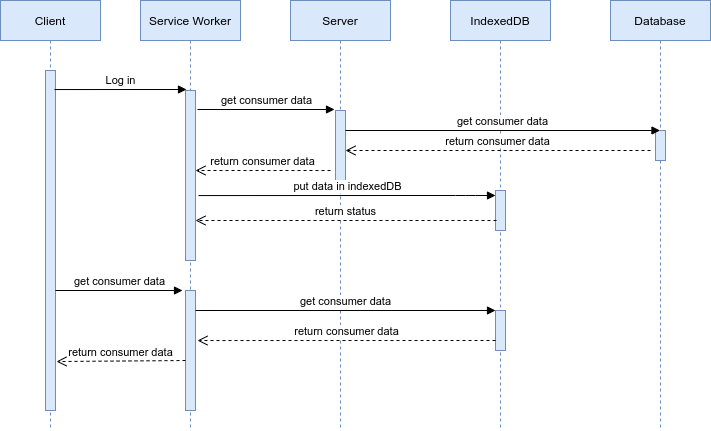
\includegraphics[width=0.9\textwidth]{images/flow}
						\label{fig:flows}
						\caption{Diagramme de séquence - chargement des données}
					\end{figure}
				
					Pour éviter d'avoir un dédoublement des données tout en conservant le principe de la base de données non-relationnelles, les données qui sont liés et qui doivent s'afficher dans la même table sont toutes regroupées dans la même collection. Cela permet de conserver une grande vitesse de lecture des données et de ne pas ralentir le fonctionnement de l'application.
							
					Pour accélérer le processus, toutes les requêtes pour récupérer les données sont envoyées simultanéments. Ainsi dès qu'une réponse est reçue, le service worker peut commencer à ajouter les données dans l'indexedDB à l'aide de la bibliohtèque "dexie.js" \cite{ref:dexie}. Pour ce faire, le service worker parcours simplement tout le fichier JSON reçu de l'API et ajoute toutes les données présentes dans la collection adéquate.
				
				\subsubsection*{Envoi des données}
					Pour gérer l'envoi des données, la première solution envisagée a été d'utiliser la nouvelle API "background-sync". Quand le service worker detecte qu'une requête réseau à échoué, il peut l'enregistrer comme un évennement sync qui sera délivré une fois que le navigateur à récupéré le réseau. 
					
					L'avantage de cette solution est que le service worker peut envoyer les données même si la page a été fermée ce qui permet d'éviter que les données restent indéfiniment non envoyées. Malheureusement cette API n'est pour l'instant prise en charge que par certain navigateur sur PC et Android mais n'est pas du tout prise en charge par iOS. Il a donc été décidé de laisser cette solution de côté.
					
					Du coup pour pallier à ce problème, j'ai implémenté une solution qui est compatible avec tous les navigateurs. Lorsque l'utilisateur essaie d'ajouter, modifier ou supprimer des données, celles-ci sont dans un premier temps stockées dans l'indexedDB avant d'être envoyées. Cela permet en cas de perte de connexion au réseau internet, de ne pas perdre les données que l'utilisateur vient d'encoder. Une fois enregistrées dans l'indexedDB, le service worker va automiquement essayer d'envoyer les données une première fois. En cas de réussite, les données sont supprimées de l'indexedDB et en cas d'échec d'envoi, les données restent stockées afin de pouvoir être envoyées plus tard. A chaque fois que l'utilisateur tentera de récupérer des données  sur le serveur, le service worker va d'abord essayer d'envoyer toutes les données en attente avant de récupérer les données du serveur. Cela permet d'éviter d'avoir des données non envoyées qui restent  en attente.
					
					Si l'envoi des données réussi, le serveur répond avec les nouvelles données mises à jour. Lorsque le service worker reçoit cette réponse, il va mettre à jour les données qui sont dans le navigateur afin que l'utilisateur puisse voir directement les changements qui ont été éffectués même s'il utilise le mode hors-ligne de l'application \ref{fig:flows2}. La gestion des incohérence sera décrite plus loin dans la section \ref{sec:api}.
					
					\begin{figure}[H]
						\centering
						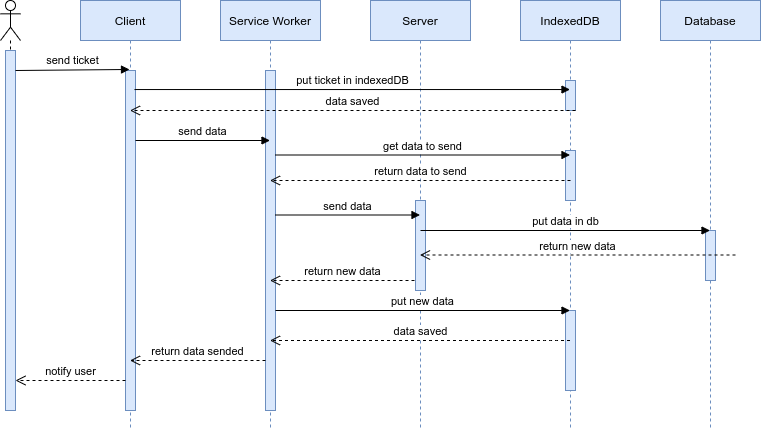
\includegraphics[width=0.9\textwidth]{images/flow2}
						\label{fig:flows2}
						\caption{Diagramme de séquence - envoi de données}
					\end{figure}
			
			\subsection{Gestion des changements d'utilisateurs}		
				Afin de conserver une sécurité maximale, à chaque déconnexion d'un utilisateur, toutes les données et les fichiers (hors fichiers statiques) sont supprimés du navigateur. Il aurait été possible de ne pas supprimer ces données et de gérer des fonctionnalités multi-utilisateurs mais cela aurait impliqué de demander à l'utilisateur d'effectuer des démarches supplémentaires pour supprimer ces données. 
			
				De plus à l'heure actuelle chaque utilisateur possède son propre appareil et il n'est donc pas nécessaire de gérer le multi-utilisateur au détriment de la sécurité. En effet si on décide de laisser les données dans le navigateur même après la déconnexion d'un utilisateur, les données restent accessible via l'inspection du navigateur. Du coup si une personne mal intentionnée  passait sur l'appareil après d'un utilisateur, il pourrait récupérer toutes les données qu'il souhaite. 
				
			\subsection{Sytème de notification}
				Le système de notification, comme indiqué dans le tableau \ref{fig:moscow}, ne faisait pas partie des fonctionnalités à implémenter pour l'instant. Toutefois, un petit système de notification local a tout de même été mis en place pour notifier l'utilisateur lorsqu'il y a des données qui sont en attente d'envoi dans le navigateur. Cela afin que ces données ne restent pas en attente indéfiniment.
		
		
		\section{Interface utilisateur}
			L'interface utilisateur existante a du subir quelques modifications afin de pouvoir accueillir le mode hors-ligne. La nouvelle application permet en effet deux modes différents d'utilisations.
			
			\subsection{Changement de mode}
				Afin de passer d'un mode d'utilisation à l'autre un bouton de mode à été ajouté en haut de l'interface à coté de la cloche de notification. Quand ce bouton affiche un rond vert, cela signifie que l'on se trouve dans le mode online de l'application. Lorsque le rond est noir alors ça signifie que l'application est en mode offline.
				
				 A coté de ce bouton de changement de mode a été ajouté un bouton permettant de mettre à jour toutes les données présentes dans le navigateur. Cela afin de ne pas obliger l'utilisateur à mettre à jour toutes les tables une par une. Juste à droite de ce bouton, on peut lire la date et l'heure des données les plus anciennes présentes dans le navigateur. Si il n'y pas de données chargées, par example quand on lance l'application pour la première fois, alors on pourra lire la phrase "Pas encore de données". Cela permet à l'utilisateur de savoir à quel point les données du navigateur sont à jour ou non.
				
				\begin{figure}[H]
					\centering
					
\includegraphics[width=0.5\textwidth]{images/buttons}
					\label{fig:buttons}
				\end{figure}
			
			\subsubsection*{Mode online}
				Il s'agit du mode par défaut lorsque l'on se connecte pour la première fois à l'application. Il faut du temps à toutes les données pour se charger dans le navigateur afin que l'application puisse fonctionner en mode hors-ligne. Du coup mettre ce mode-ci par défaut permet à  l'utilisateur de déjà utiliser l'application en attendant que les données soient bien toutes chargées. Dans ce mode les différentes pages vont aller récupérer les données à afficher directement dans la base de données grâce à l'API et pas dans l'indexedDB du navigateur. 
				
				Ce mode est très utile lorsque l'on a besoin d'avoir les dernières données disponible et que le réseau le permet. Si vous désirez plus d'information sur ce mode de fonctionnement vous pouvez consulter le mémoire de la première version de l'application \cite{ref:haitiwater}.
			
			\subsubsection*{Mode offline}
			
				Ce mode permet d'afficher les données qui sont présentes localement dans l'indexedDB du navigateur. C'est dans ce mode que l'utilisateur pourra utiliser l'application lorsque la connexion au réseau internet n'est pas disponible. Lorsque l'on passe dans ce mode, la couleur du bandeau de l'application change pour passer du bleu au rouge et ce afin d'indiquer qu'on est bien dans le mode hors-ligne, voir \ref{fig:mode}, et que les données ne sont pas récupérées directement sur le serveur.
								
				\begin{figure}[H]
					\caption{Mode}
					\label{fig:mode}
					\centering
					\begin{subfigure}[b]{0.3\textwidth}
  						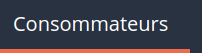
\includegraphics[width=1\linewidth]{images/consumer_blue}
  						\caption{Online}
					\end{subfigure}%
					\begin{subfigure}[b]{0.333\textwidth}
  						
\includegraphics[width=1\linewidth]{images/consumer_red}
  						\caption{Offline}
					\end{subfigure}
					\label{fig:test}
				\end{figure}
			
				Dans ce mode, lorsque du travail sur des de données n'a pas pu être envoyé, les données concernées apparaitrons en mauve dans le tableau pour que l'utilisateur sache que des modifications sont en attente sur celles-ci. Une fois que les données ont pu être envoyées et que le serveur à répondu un status 200, les données hors-ligne que nous avons modifiées sont mise à jour localement pour refléter les changements faits sur le serveur et ces données n'apparaissent du coup plus en mauve dans les tables, voir \ref{fig:purple}. 
				
				\begin{figure}[H]
					\centering
					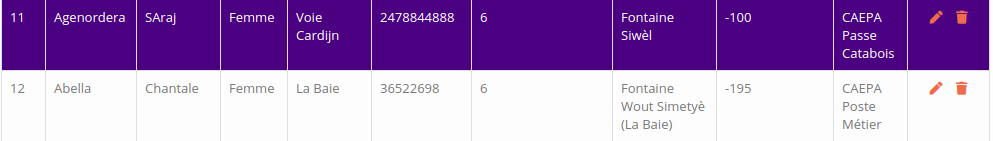
\includegraphics[width=1\textwidth]{images/purple}
					\caption{Donnée pas synchronisée}
					\label{fig:purple}
				\end{figure}
							
			\subsection{Module à synchroniser}
				Il s'agit d'un nouveau module qui a été ajouté pour les besoins du mode hors-ligne. Dans ce module, l'utilisateur pourra retrouver un tableau qui contient toutes les données qui n'ont pas étés envoyées vers le serveur. Dans ce tableau, il peut retrouver différentes informations, voir \ref{fig:tosync}.
				
				\begin{figure}[H]
					\centering
					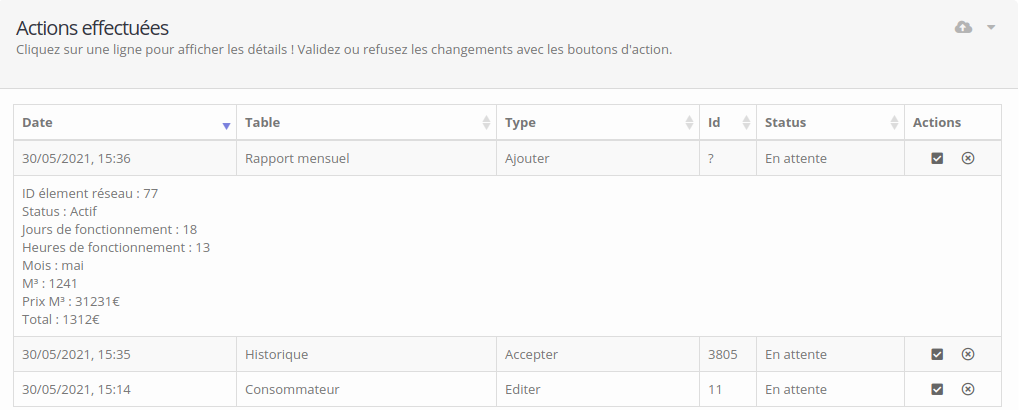
\includegraphics[width=1\textwidth]{images/tosync}
					\caption{Module à synchroniser}
					\label{fig:tosync}
				\end{figure}
							
				L'utilisateur peut choisir de supprimer des données du tableau, auquel cas il ne pourra plus essayer de les envoyer car celle-ci seront supprimées de l'indexedDB. Ou bien il peut choisir d'essayer d'envoyer une donnée en particulier ou toutes en même temps avec le bouton prévu dans cette optique dans l'entête du tableau.
			
		
		\section{Serveur}
		\label{sec:serveur}
			Dans cette partie je vais décrire le fonctionnement du serveur. Je ferai d'abord un petit résumé sur le fonctionnement de base du serveur et ensuite j'expliquerai les changements que j'ai apporté au serveur afin de récupérer les données nécessaires à l'affichage hors-ligne.
			
			\subsection*{Requêtes}
				Une réquête est une demande que le navigateur envoi au serveur afin de récupérer différents type fichiers ou de données. Le serveur permet de gérer trois types de requêtes différentes :
				
				\begin{description}
					\item[Fichiers statiques.] Le serveur répond a ces requêtes en envoyant tous les fichiers CSS et Javascripts.
					\item[Documents.] Le serveur renvoie les pages HTML à afficher à l'utilisateur. Ce sont les documents qui vont importer les fichiers statiques.
					\item[Données.] Le serveur renvoie toutes les données demandées. Pour ce faire, on utilise l'Object-relational mapping. Django se charge d'effectuer la connexion avec la base de données et de lui renvoyer toutes les requêtes. Cela permet d'intéragir avec les données sans avoir à toucher au SQL.
				\end{description}

				Les fichiers statiques et les documents permettent au navigateur d'afficher toute l'interface graphique. Chaque module du serveur permet de desservir une page de l'application. Ces pages peuvent avoir des éléments personnalisés en fonction de l'utilisateur connecté. Les données elles sont téléchargées après le chargement de la page. Toutes ces données sont récupérées via le module API du serveur. Cela permet de mieux gérer la séparation des rôles. 		
				
				Le fonctionnement global du serveur n'a pas été modifié car ce n'est pas sur cette partie que portait ce mémoire.
				
			\subsection*{API}
				\label{sec:api}
				Le module API a subit quelques modifications afin que le service worker puisse télécharger toutes les données dont il a besoin lorsque la connexion au réseau n'est pas disponible. La version de base du serveur ne permettait que de télécharger une partie des données, celle à afficher directement par la page. Par exemple, lorsque l'application doit afficher la page consommateur, l'API ne répond que les 10 éléments doivent être affichés sur la page et une nouvelle requête est nécessaire à chaque fois que l'on veut voir des données différentes (la page 2 du tableau par exemple).
				
				Pour résoudre ce problème, j'ai implémenté des fonctions supplémentaires qui permettent de récupérer en une seule requête toutes les données nécessaires à l'affichage d'une table. Cela permet au service worker de récupérer toutes les données dont-il a besoin afin de les sauvegarder dans l'indexedDB lors de l'installation de celui-ci. Bien sûr ces nouvelles fonctionnalités demandent tout de même à l'utilisateur d'être connecté avec un compte utilisateur valide pour pouvoir récupérer les données.
				
				De plus afin d'aider le mode offline à être plus précis dans l'affichage des données, lorsque qu'une demande d'ajout, de modification ou de suppression de données, le serveur ne vas pas juste répondre avec un status 200, qui signifie que les changements ont bien été pris en compte, mais il va également renvoyer la donnée modifiée au format JSON afin que le service worker puisse mettre à jour directement les données localement. Le JSON est un format de données textuelles qui permet de représenter l'information sous forme de texte. 
				
				Une autre problématique est que lorsque que les utilisateurs ne sont plus connectés au réseau internet, il est possible qu'ils modifient à des moments différent la même donnée. Vu que pour l'instant le travail des gestionnaires de fontaines doit être validé par un gestionnaire plus haut placé via le module "Historique" décris au point \ref{sec:historique}, le serveur va simplement accepter les données comme elles viennent et les ajouter dans la liste des données qui doivent être validées. Comme ça si des incohérences apparaisent, la gestionnaire responsable peut contacter les gestionnaires concernés par l'incohérence et la corriger et approuvant ou rejetant les modifications faites. Pour l'instant la donnée qui apparait sur le serveur est celle de l'utilisateur qui a envoyé ces données en dernier.
			

	\chapter{Validation}
		La validation a pour objectif de tester le bon fonctionnement et le niveau de qualité du produit "fini". Pour effecuter cette validation, deux types de tests ont été utilisés. D'abord des tests automatisés afin de pouvoir tester le fonctionnement des différentes fonctions implémentées. Et ensuite des tests  de validation avec des utilisateurs réels afin de tester le fonctionnement global de l'application ainsi que son intuitivité.

		

		\section{Vérifications automatiques}
			Pour tester l'application de façon automatique, j'ai utilisé des tests unitaires. Ces tests ont pour objectif de vérifier le bon fonctionnement d'une petite partie bien précise d'une application (unité ou module). Ils assurent qu'une méthode qui peut être utilisée par un utilisateur fonctionnent bien de la manière prévue. Dans le cas présent, toutes les intéractions entre l'utilisation et l'utilisateur se font à l'aide soit de requêtes envoyées directement au serveur, soit de requêtes faites au service worker. J'ai donc décider de compléter les tests unitaires qui étaient déjà présent pour la partie serveur et de créer un batterie de tests unitaires pour le service worker.

			Si vous voulez connaitre les détails des tests unitaires déjà présent de base vous pouvez consulter le mémoire en lien avec la création de l'application \cite{ref:haitiwater}. Les tests que j'ai rajouté au niveau des reqûetes au serveur couvrent les méthodes de récupération des données utilisées par le service worker. Je vérifie que les données récupérées sont bien uniquement celles auxquelles l'utilisateur à accès et que celles-ci sont bien complète.
			
			En ce qui concerne les tests sur le service worker, ceux-ci couvrent toutes les fonctions de récupération et d'envoi de données depuis et vers la base de données ainsi que la gestion de toutes pages mises en cache pour leur affichage en mode hors-ligne.

		\section{Vérifications utilisateurs réels}
			Lors de cette phase, des utilisateurs qui avaient déjà ou non testés la première version de l'application se sont retrouvés face à celle-ci pour la tester. Pendant ces tests, trois choses étaient testées: la compréhension des différents mode, la gestion des données en cas de perte de connexion et les modifications de l'interface. Le fait d'avoir des avis externes sur l'application peut permettre de l'améliorer drastiquement.
			
			% Marion
			% 2 officiels
			% 2 Nahomie
			% Sarah
			% Maman
			% Robin
			% Marlon
			% Guillaume
			
			Les tests se sont déroulés en direct avec les participants ou via teams en fonction de la disponibilité des personnes et des règles de la période COVID. Un groupe de 10 personnes venant d'horizons différentes et avec des compétences diverses et variées ont testés l'application.


			\subsection*{Méthodologie}
				La méthodologie qui a été utilisée pour faire passer ces tests est restée la même que pour le mémoire précédent \cite{ref:haitiwater}. Celle-ci a été adaptée aux nouvelles fonctionnalités développées lors de ce mémoire afin que ce test reste cohérent avec le travail réalisé. Le fait de réutiliser le même type de test permet de voir concretement comment évolue le niveau de satisfaction des utilisateurs après cette deuxième année de développement.
				
				Les séances de validation se sont déroulées en partie physiquement et en partie à distance via les logiciels Teams et Zoom, ces logicielles permettant de faire de la transmission vocale et du partage d'écran. L'étudiante d'Haïti m'a également aidé à faire passer les tests aux différentes personnes qui étaient présentes la-bas, cela afin de me faciliter la tâche à cause du décalage horaire.
				
				Les testeurs ont d'abord reçu une brève introduction sur l'application et elle même et sur le but de la séance de validation. Je leur ai ensuite remis un ou deux scénarios à réaliser durant la séance. Ces scénarions contiennent une brève introduction au contexte et une liste de tâches à compléter. Après la lecture du scénario, je laissais au testeur quelques minutes au cas où il aurait des question à poser sur le scénario. Ensuite l'utilisateur est laissé seul pour faire sa tâche et est chronométré. Si celui-ci avait des questions pendant le déroulement de la tâche, celui-ci pouvait recevoir une indication pour l'aider à accomplir sa tâche.
				
				Une fois que le testeur avec executé entre 1 et 3 scénario en fonction de la disponibilité du celui-ci, une série de 18 questions lui étaient posées. Ces questions sont regroupées par thème. Ces quatres thrèmes sont :
				\begin{description}
					\item[Tâches.] Ces questions permettent de savoir si les tâches à accomplire étaient suffisament claire.
					\item[Fonctionnalités.]  Ces questions servent à savoir si l'interface de l'application permet une utilisation simple des fonctions implémentées.
					\item[Usabilités.] Ces questions permettent d'avoir le ressenti plus subjectif de l'utilisateur. Cela permet des indices quand à une possible amélioration de l'application au niveau l'utilisabilité.
					\item[Esthétique.] Ces question permettent de savoir si le design de l'application plaît aux utilisateurs.
				\end{description}

				Pour répondre aux différentes questions, j'ai utilisé l'échelle de Likert. L'échelle de Likert est une échelle de mesure qui comprend dans ce cas 5 dégrés de réponse. Elle est souvent utilisée dans les questionnaires. Elle permet de jauger le niveau d'accord ou de désacord d'une affirmation \cite{ref:likert}.
				
	
			\subsection*{Résultats obtenus}
				
			
			
			.
Les résultats des 14 questions évaluant la satisfaction des utilisateurs sur le
concept, les fonctionnalités et l’esthétique de l’application sont représentés en
figure 6.1.
Nous pouvons constater une tendance positive dans les réponses aux questions
ainsi qu’une cohérence dans les groupements : les quatre questions ayant reçu le
score le plus bas sont toutes liées à une certaine complexité de l’interface.
Les dix questions de la SUS s’évaluent différemment. L’échelle a sa propre
formule de calcul [3] qui permet de normaliser les résultats à une valeur de 0 à
100. Notez cependant qu’il ne s’agit pas d’un pourcentage de qualité mais d’une
valeur suivant une distribution gaussienne dont la moyenne empirique se situe à 68.

				En attente dans interview de Nahomie.
				


%------------------------------------------------------------------------------------------------------
	\chapter{Améliorations futures}
		Malgré les deux années de travail passées sur ce projet, d'abord pour les 3 anciens mémorants \cite{ref:haitiwater} et ensuite par moi-même, celui-ci est loin d'être terminé. Même si l'application peut commencer à être deployée dès maintenant, comme tout gros projet de développement, HaïtiWater va devoir être suivi afin d'être mis à jour et maintenu pour un bon fonctionnement au quotidien. 

		\section{Suite du projet}
			\label{ref:suite_projet}
			Faire la finition d'HaïtiWater sera la priorité des futures équipes de développement. Dans son état actuel, l'application peut déjà servir aux acteurs locaux afin de travailler sur le terrain. Mais la base de l'application pourrait toujours être optimisée pour être encore plus réactive et sûre.		
			
			Une des tâches importantes pour le futur, reste comme l'avait dit mes prédécesseurs \cite{ref:haitiwater}, d'automatiser les rapports en aggrégant les données et en trouvant une bonne façon de visualiser celles-ci. Ils proposaient également d'avoir dans le futur un serveur mail dédié afin de ne pas bloquer le serveur de l'application lorsque celui-ci doit envoyer des mails via le système de mailing inclu avec Django et pourquoi pas mettre en place un serveur de SMS.
			
			L'application HaïtiWater est en cours de déploiement sur un serveur Haïtien et devrait être disponible dans les semaines à venir. Cette migration devrait améliorer le temps de chargement de l'application pour les acteurs locaux. Le serveur qu'ils utiliseront devrait d'ailleurs être plus performant que celui utilisé en Belgique. Pour l'instant il s'agit d'un serveur dual-core de 2 GHz avec 2 Go de ram. Les temps de chargement devraient donc être drastiquement réduits avec un serveur plus puissant. 
			
			Une dernière chose à faire serait d'optimiser les requêtes faites à la base de données pour récupérer les informations des consommateurs. Actuellement, c'est la raison pour laquelle l'application prend du temps à être complétement chargée pour une utilisation hors-ligne. C'est également ce délai qui empêche l'utilisation du mode hors-ligne avec Firefox pour les gestionnaires qui ont beaucoup de consommateurs dans sous leur responsabilités. Le problème étant que Firefox stoppe le service worker bien avant d'avoir reçu la réponse du serveur.
			

		\section{Défis rencontrés}
			La plus grosse difficulté lors de se projet a été la méconnaissance de la technologie utilisée et le fait qu'il y ai encore peu de documentation trouvable sur le net. De plus les services workers sont encore en cours de développement et toutes leurs fonctionnalités ne sont donc pas supportées par tous les navigateurs. Il a donc fallu trouver des solutions pour que l'application puisse rester fonctionnelle même si l'utilisateur emploie un navigateur qui ne prend pas en charge les services workers. Une grosse période d'apprentissage autonome avant de se lancer dans le projet à été nécessaire.
			
			Une autre difficulté était que c'est la première fois que je me lance seule dans un projet d'une aussi grande envergure. Heureusement les anciens mémorants étaient assez disponibles et m'ont aidé au début de celui-ci à résoudre les difficultés rencontrées.
			
			Le dernier gros défi auquel j'ai du faire face a été la période COVID-19. En effet l'isolement social et le manque d'objectif à court terme ont causé un gros manque de motivation  qu'il a fallu surmonter afin de terminer ce mémoire.
			

		\section{Propositions}
			L'application HaïtiWater peut encore évoluer de nombreuse manières. Une demande a été faite pour intéger un module Citizen Science afin que les consommateurs du réseau de distribution d'eau potable puissent signaler eux-mêmes les différents problèmes présents sur ce réseau ainsi que consulter leurs factures et consommations.
			
			Bien que l'application soit déjà bien optimisée avec la mise en cache de toutes les fichiers nécessaires à l'affichage des pages et la copie locale de la base de données, une autre amélioration possible serait d'utiliser un framework tel que vue, react ou angular afin d'améliorer la réactivité globale de l'interface. De plus ces frameworks s'intègrent parfaitement avec les Progressive Web-App.
			
			La gestion des données stockées localement pourraient être améliorée afin de ne plus proposer deux modes différents de fonctionnement de l'application mais un seul mode dans lequel toutes les données seraient synchronisées automatiquement au fur et à mesure que l'utilisateur fait des requêtes au serveur.
			
			Une autre évolution possible serait de rajouter un vrai système de notification basé sur le serveur plutôt que juste localement. Pour l'instant ce système de notification n'est pas du tout synchronisé côté serveur et ne sert que pour afficher certaines informations stockées dans le navigateur. Un service de messagerie interne à l'application pourrait également aider les utilisateurs à communiquer entre eux. Une fois ce système de notification mis en place, la gestion des incohérences de données telles que décrite dans la section \ref{sec:api} pourra être améliorée afin d'envoyer des avertissements aux deux utilisateurs qui ont modifiés les mêmes données dont un court laps de temps.
		
			Enfin, les modules déjà existants pourraient être améliorés afin de proposer différentes façon d'intéragir avec les données, par exemple en proposant de créer un fichier excel à partir de la base de données ou bien intégré plus d'outil graphique pour rendre les informations plus visuelles et ainsi offrir une personnalisation plus poussée de l'affichage.


			
	\chapter{Conclusion}
		Voici donc finalement la conclusion de ce mémoire qui met aussi fin au plus gros projet sur lequel j'ai eu l'occasion de travailler durant toutes mes études. Ce travail m'aura permis d'utiliser toutes les compétences acquises pendant toutes ces années. Il m'a également apporté une expérience non négligeable dans le développement d'une application web de grosse envergure.
		
		Durant la validation avec de vraies personnes, l'application et son nouveau mode hors-ligne a eu l'air de susciter beaucoup d'intérêts chez les testeurs et les retours étaient plûtot positif. J'ai bon espoir qu'HaïtiWater finira par être utilisée par les acteurs locaux Haïtiens de façon régulière et j'espère que celle-ci va continuer à évoluer avec le temps. 
		
		J'espère qu'au même titre que les personnes qui ont testés l'application, les acteurs de Protos et d'Haïti trouveront que cette nouvelle version de l'application simple d'usage et suffisament pratique que pour être utilisée tous les jours sur le terrain. 

		

	\bibliographystyle{plain}
	\bibliography{bibliography.bib}
		

	

	\setlength{\parskip}{0em}
	\backcoverpage

\end{document}
